\documentclass[referee,a4paper,12pt]{swsc}

\usepackage{graphicx}
\usepackage{txfonts}
\usepackage{subfigure}
\usepackage{epstopdf}
\usepackage{lineno}
\usepackage[authoryear,round]{natbib}
\usepackage[backref]{hyperref}
\usepackage{url}
\bibliographystyle{plainnat}
\hypersetup{colorlinks=true,citecolor=cyan,urlcolor=cyan,linkcolor=blue}

\author{Andrew Leonard*
        \and Huw Morgan}

\institute{Institute of Mathematics, Physics and Computer Science, Aberystwyth University, Ceredigion, SY23 3BZ, Wales\\
					 \email{\href{mailto:ajl7@aber.ac.uk}{ajl7@aber.ac.uk}}}

\title{Using temperature distributions of active regions to investigate flare activity}

\begin{document}

\begin{linenumbers}

\titlerunning{Temperature distributions of active regions}
\authorrunning{Leonard and Morgan}
% {}{Aims}{Methods}{Results}{}
\abstract
	{}
	{To investigate whether signatures of solar flares can be seen in the temperature distributions of flaring active regions before the flares occur.}
	{A recently developed and extremely fast temperature-mapping method is used to determine the temperature of flaring active regions for the 30 minutes preceding a flare.}
	{No clear link was found between active region temperature and flare activity. However, the distribution of active region mean temperatures does suggest that a much larger sample size might show some relationship between this and peak flare flux.}
	{}
\keywords{}

\maketitle

%===========================================================================
\section{Introduction}
Solar flares are a complicated and as yet not fully understood phenomenon.
In particular, growing emphasis has been placed in recent years on studying how to predict when a flare will occur, since flares and associated coronal phenomena can have significant detrimental effects on a variety of modern electronic infrastructure.
Many studies have been devoted to this topic (eg, \citealt{Korsos2014, Ahmed2011, Bloomfield2012}, etc.), but few have looked at the temperature of the active regions associated with flares before the flare occurs.

Studying the temperature of the corona is not a new pursuit, but for many years the data were significantly limited.
Most imagers had either relatively poor spatial resolution or too few wavelength channels to effectively constrain temperature solutions, whereas spectrometers could provide very accurate temperatures but only over very small portions of the corona.
Imagers and spectrometers also typically had insufficient temporal resolution to investigate any dynamic events in the corona.
Recently, however, the very high temporal and spatial resolution of the Atmospheric Imaging Assembly (AIA) on the Solar Dynamics Observatory (SDO) allows us to investigate small-scale and dynamic events anywhere on the solar disk at any time.
The six Fe-based EUV channels of AIA also provide sufficent constraints to allow a reasonable estimate of coronal temperatures \citep{Guennou2012, Guennou2012a}.

This work makes use of the capabilities of AIA in order to investigate the temperature distributions of several flaring active regions.
The aim is to search for a common signature of flare activity in these temperature distributions before flares occur, which, if found, could form the basis of a flare prediction algorithm.
To achieve this, we look at temperature distributions of the active regions over the 30 minutes before a flare occurs, and we also directly compare the temperatures of the corresponding active regions at several different before the flares.

Although it is faster than others of its kind, the temperature-calculating method used here requires a very large amount of AIA data, which can take a long time to download process.
As such this is a preliminary work investigating a relatively small number of flares and the results should not be considered definitive.
Rather they are a demonstration of the type of study made available by fast temperature analysis of the corona, which until recently has not been possible.

%===========================================================================
\section{Method}
\subsection{Temperature analysis}
The core of this analysis is the temperature map method described by \cite{Leonard} (henceforth Paper I).
Briefly, this method compares the relative brightnesses in each AIA wavelength channel at a given time and infers the best-fitting temperature from that comparison.
This allows the temperature of the corona to be estimated for every pixel of an AIA image, resulting in very high resolution temperature maps.
Crucially, this method produces temperature maps extremely quickly, which allows us to investigate coronal temperatures during localised dynamic events such as flares.
With other, slower methods, such studies are infeasible due to the computation time required.
An example temperature map is shown in Figure \ref{fig:example_tmap}.

The Paper I method also allows easy `tracking' of solar regions by cropping the temperature map around a set of Carrington heliographic coordinates, which rotate at approximately the rate of solar rotation.
This tracking is demonstrated in Figures \ref{fig:trackdemo1} and \ref{fig:trackdemo2}, each of which shows a cropped region of an AIA 17.1nm image containing active region AR11158, the corresponding temperature map and a larger 17.1nm image showing the location of the region in the corona.

\begin{figure}
	\centering
		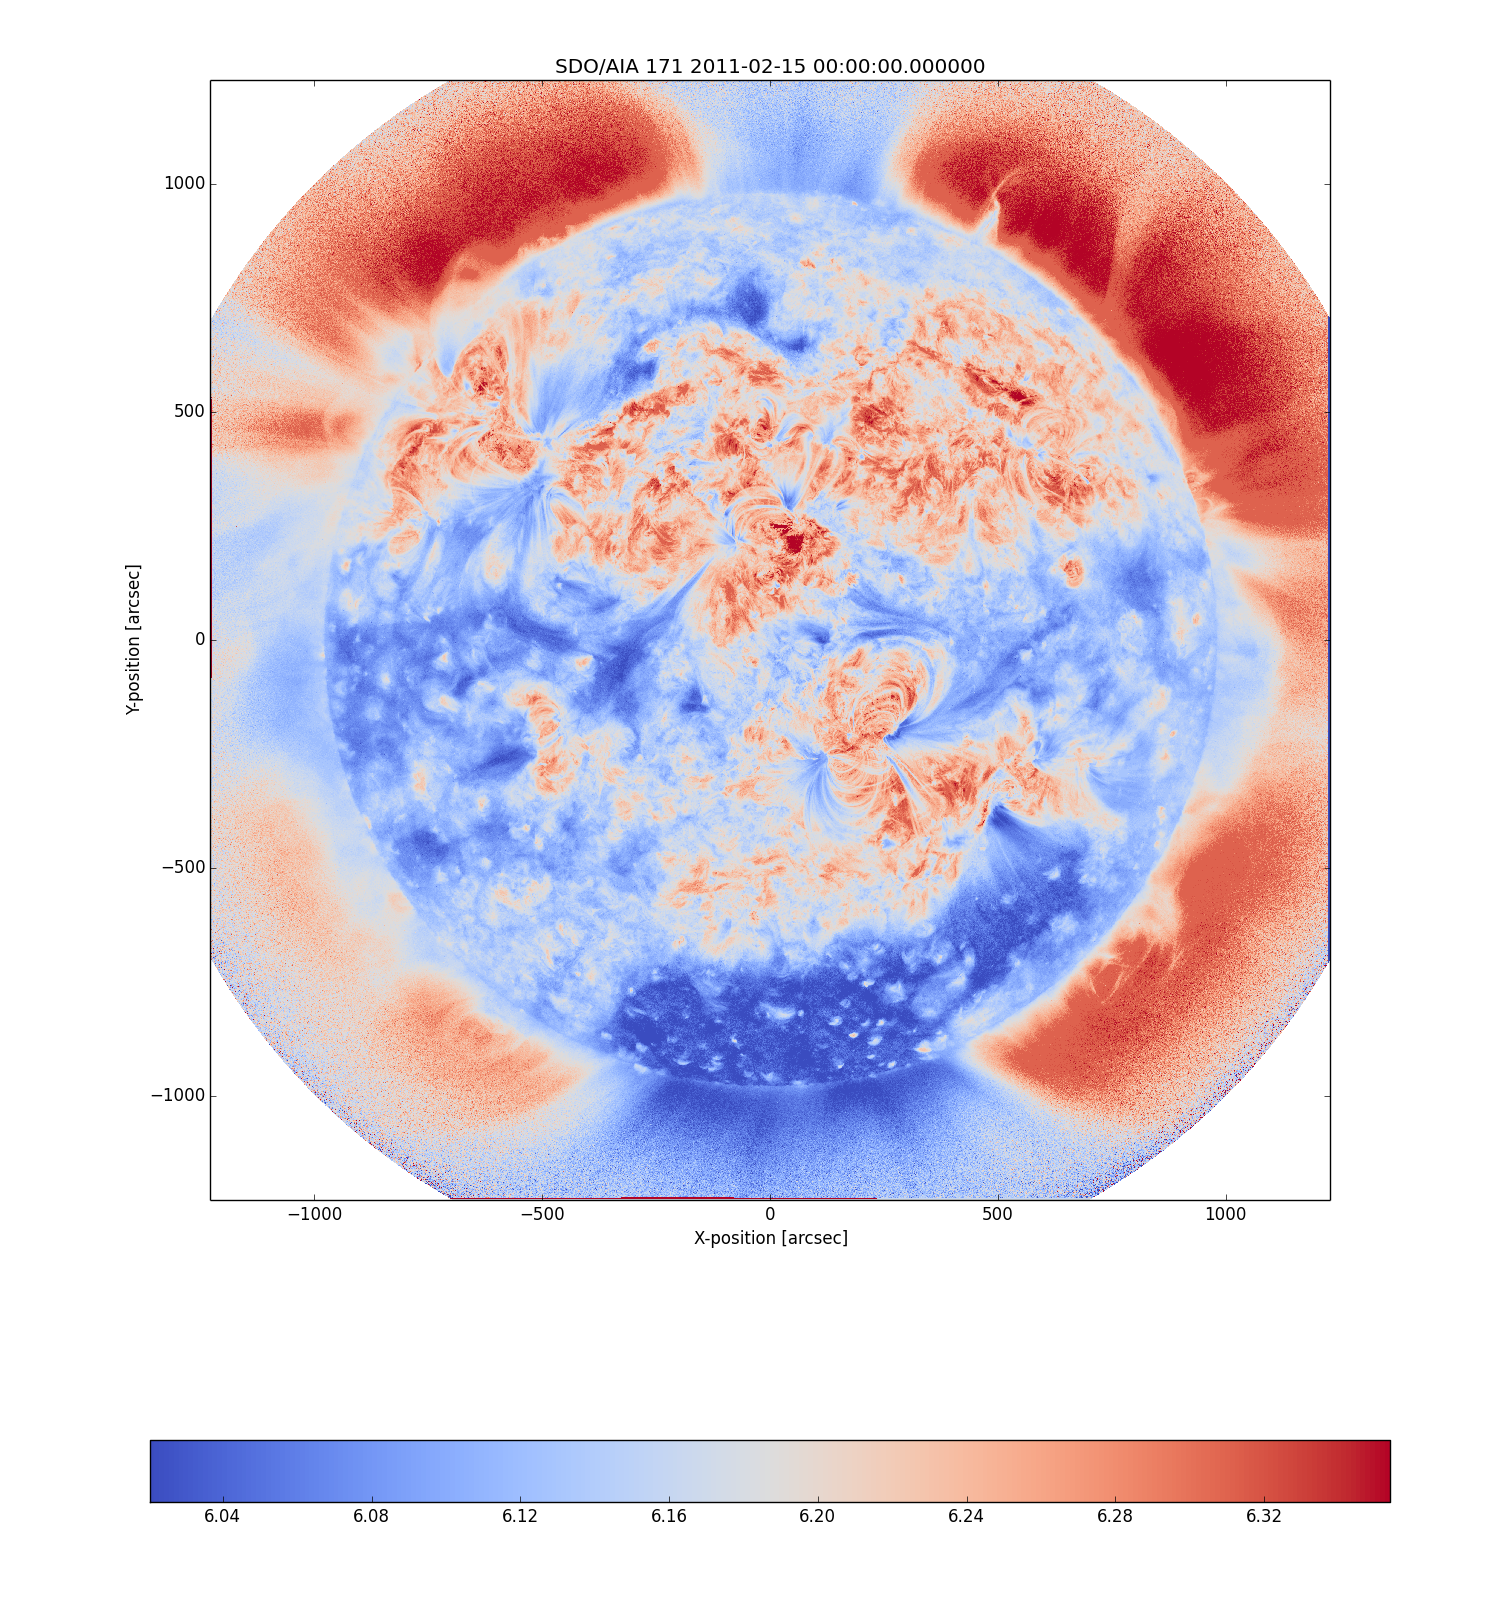
\includegraphics[width=\columnwidth]{2011-02-15T00_00_00.png}
	\caption{Example temperature map for the full solar corona at 2011-02-15 00:00}. Temperatures are displayed on a logarithmic scale.
	\label{fig:example_tmap}
\end{figure}

\begin{figure}
	\centering
		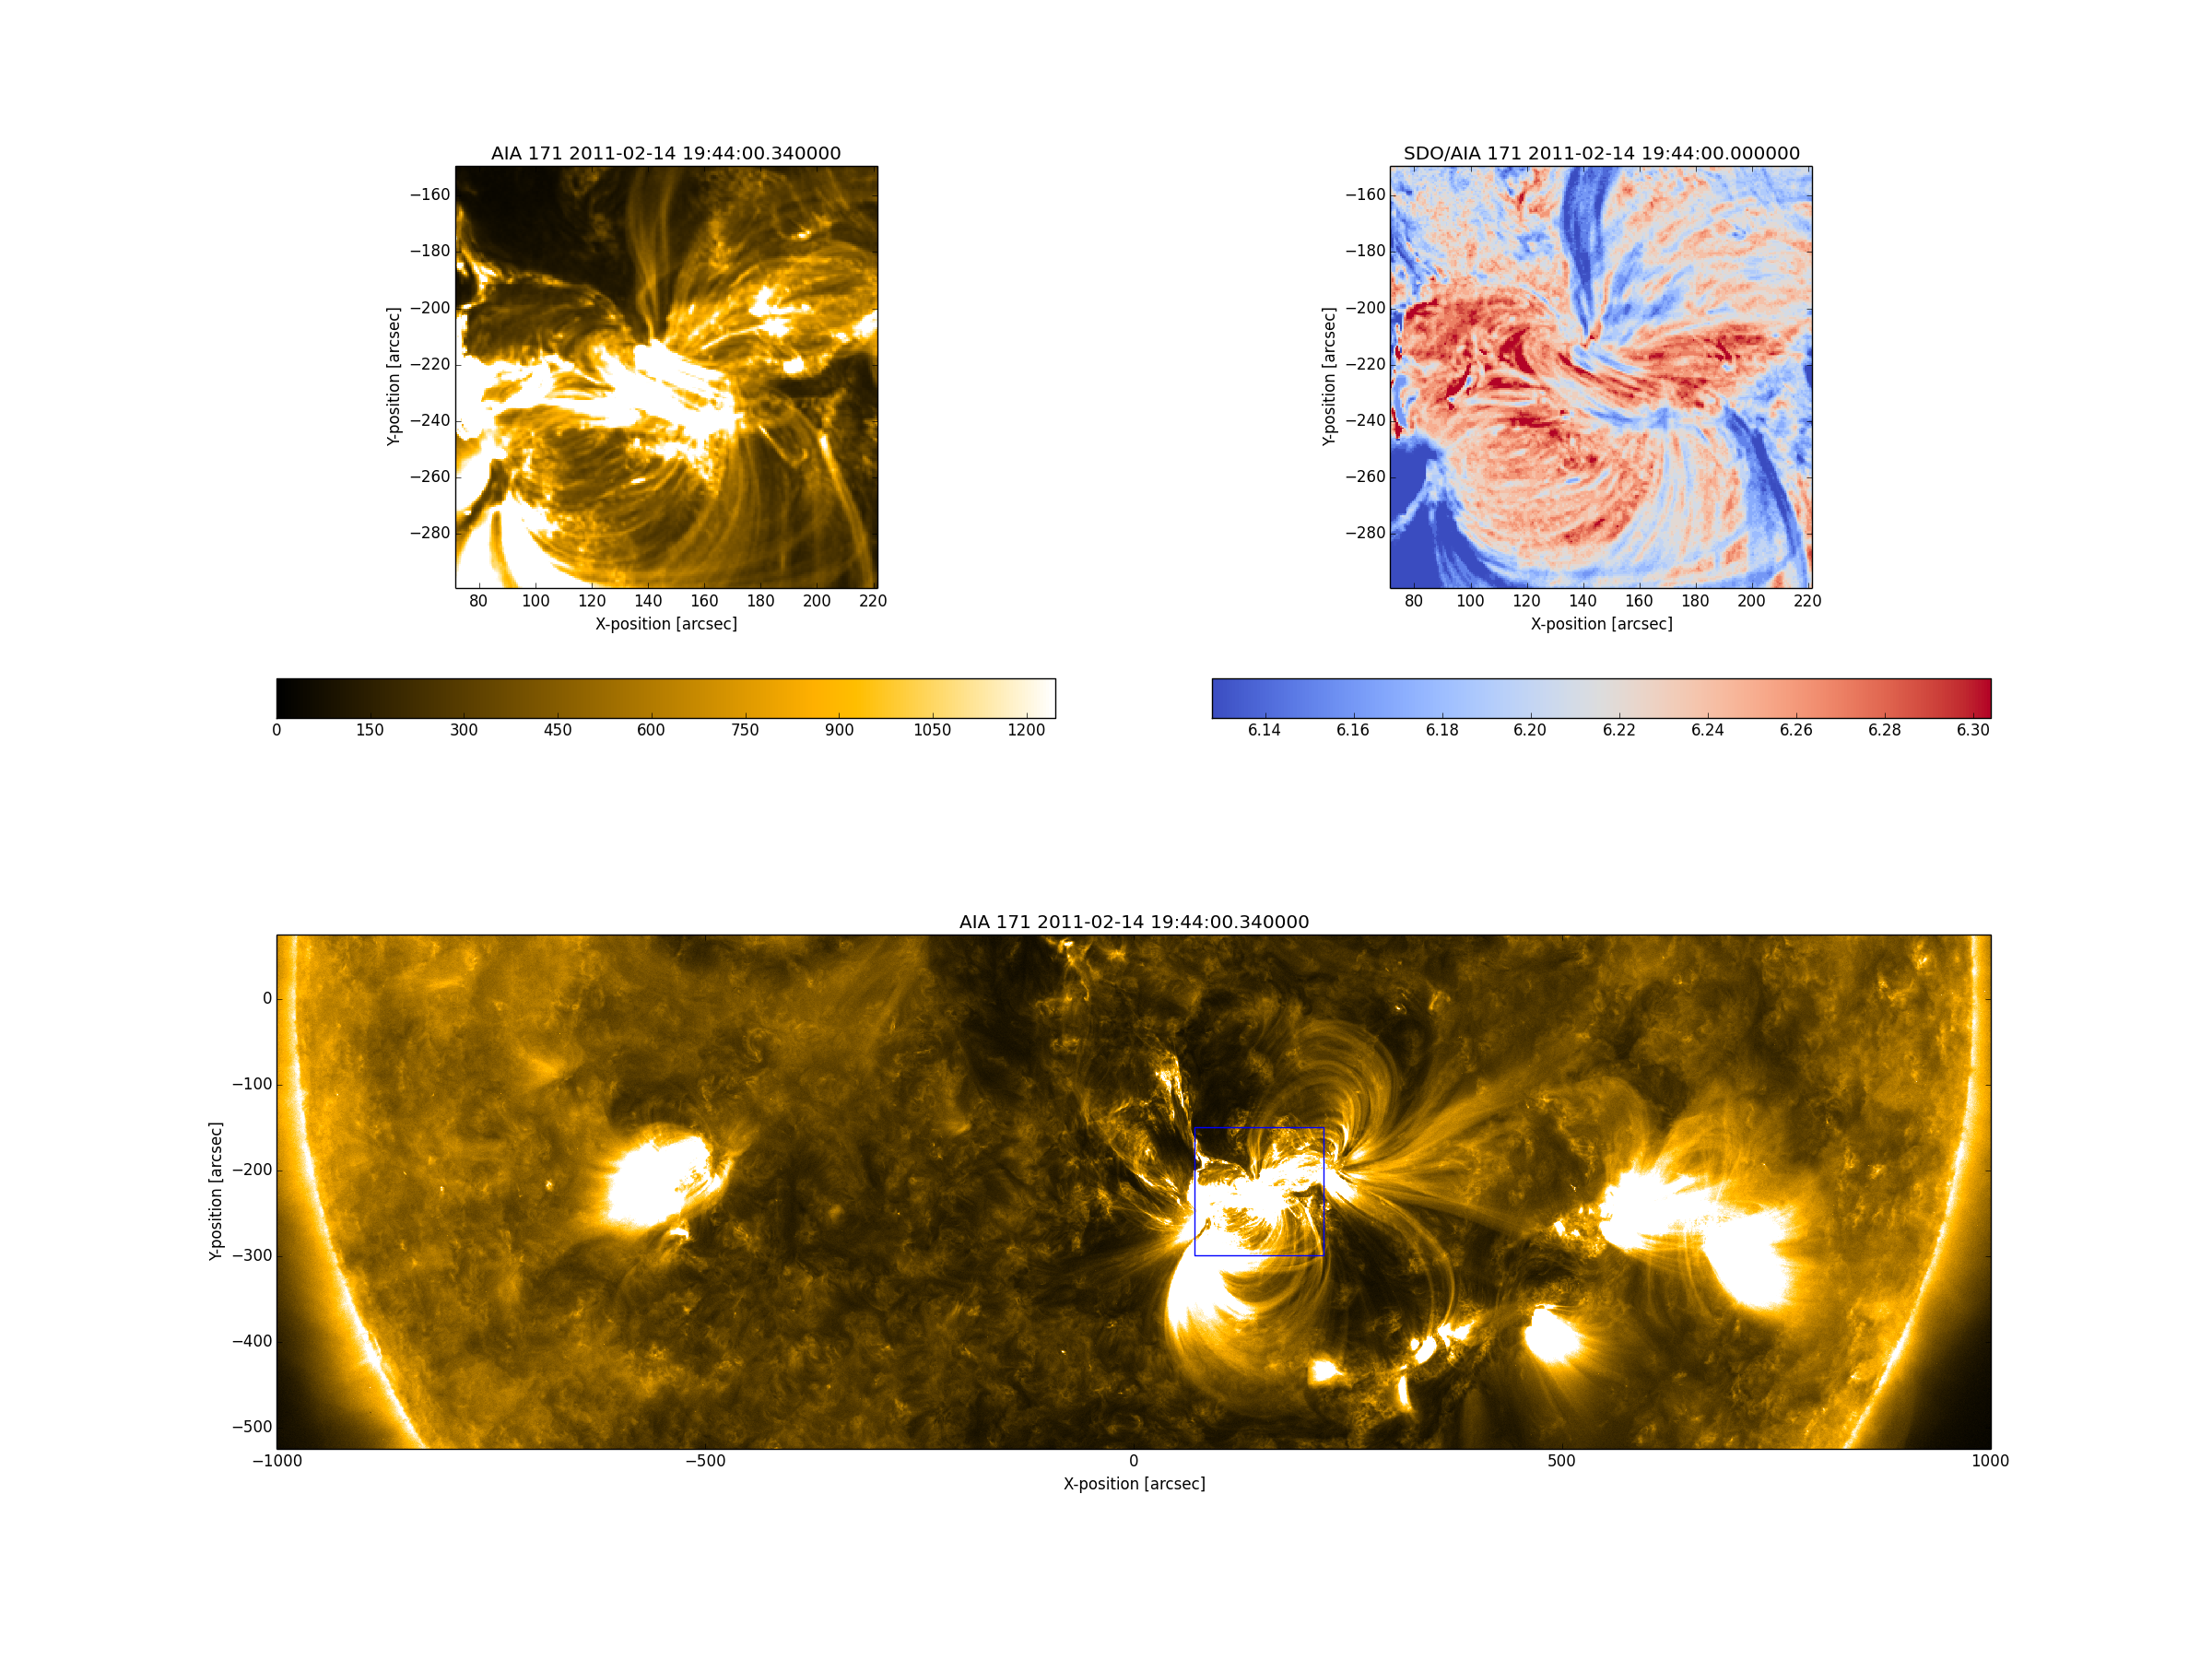
\includegraphics[width=0.9\columnwidth]{20110214T194400with171.png}
	\caption{Top left: Cropped 17.1nm AIA image showing active region AR 11158 at 2011-02-14 19:44:00. Top right: temperature map of active region AR11158 at 2011-02-14 19:44:00. Bottom: Larger 17.1nm image; the blue square outlines the region shown in the top images.}
	\label{fig:trackdemo1}
\end{figure}
\begin{figure}
	\centering
		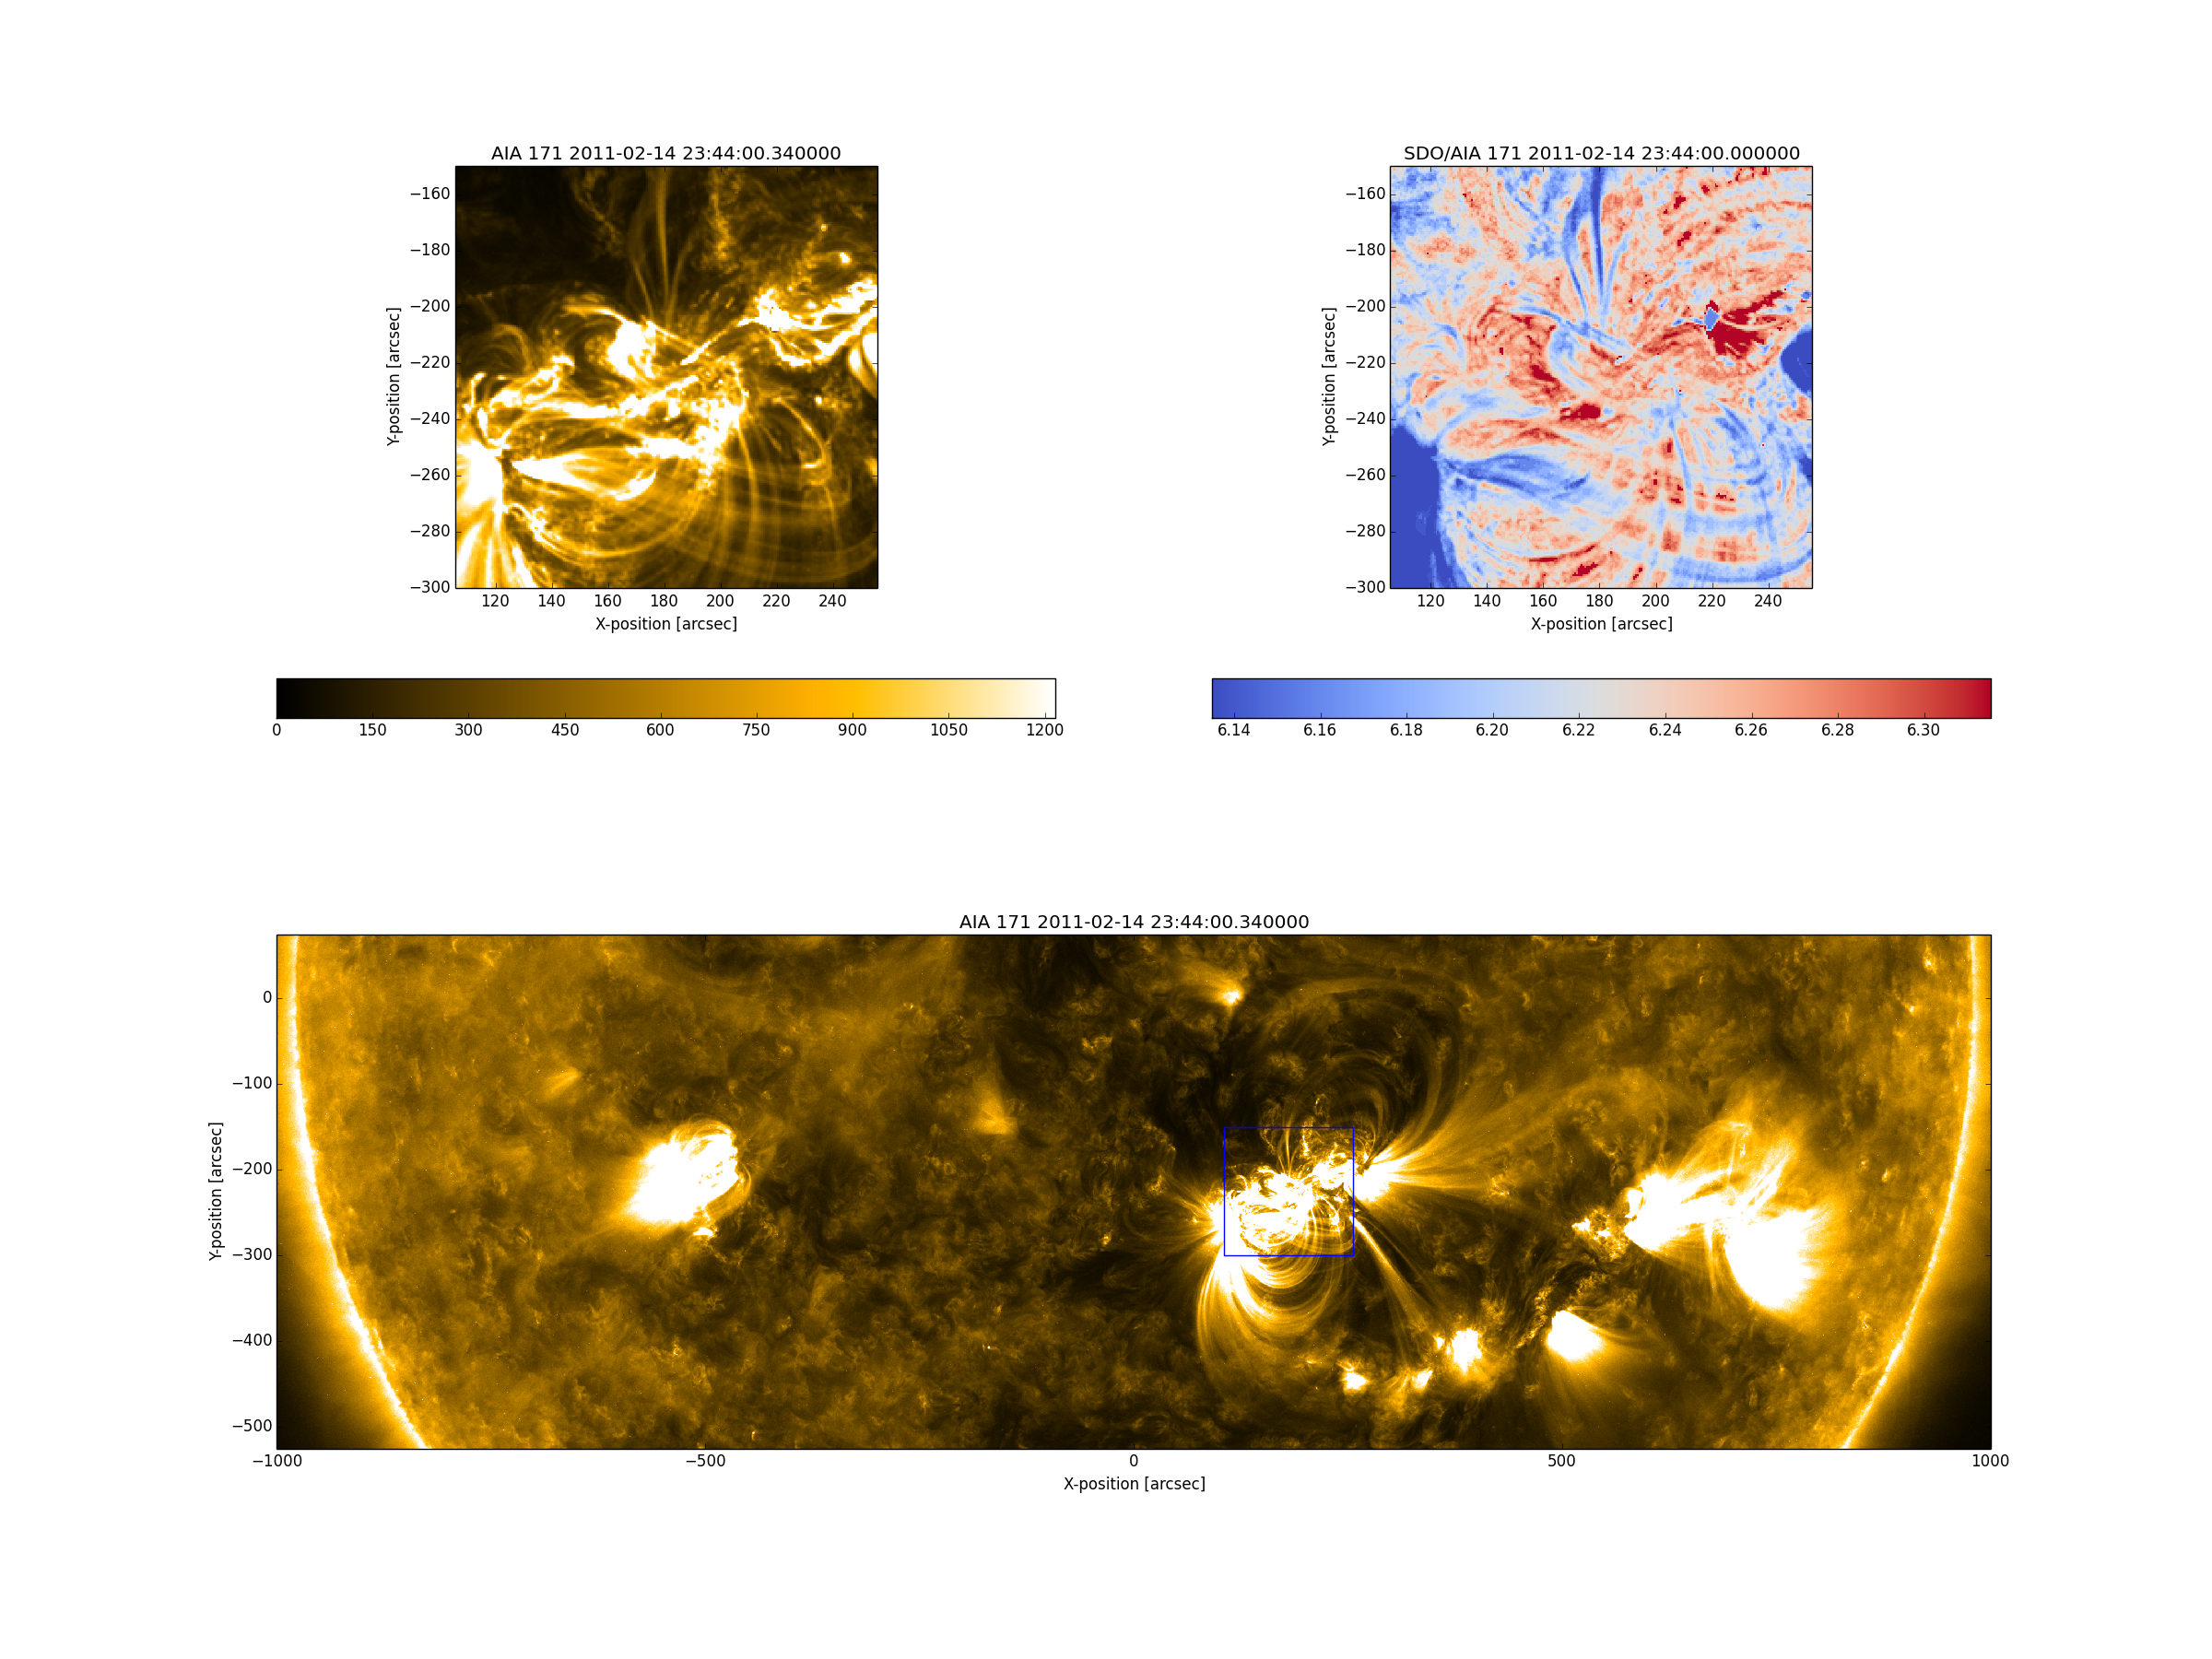
\includegraphics[width=0.9\columnwidth]{20110214T234400with171.png}
	\caption{The same images as Figure \ref{fig:trackdemo1} for time 2011-02-14 23:44:00.}
	\label{fig:trackdemo2}
\end{figure}

\subsection{Active region analysis}
The temperature map method described in Paper I was used to investigate the temperatures of the active regions associated with flares which occured during February 2011.
This month was chosen because several flares occured during this time with a wide range of peak fluxes.
The flares detected included many small flares (B and C class) as well as several larger M class flares and a single X class flare.

For each flare event investigated, a temperature map was calculated for a 150 x 150 arcsec area around the corresponding active region at 1-minute intervals for the 30 minutes preceding the start of the flare.
The maximum, 95th percentile, mean, 5th percentile and minimum temperatures were then calculated for each temperature map for each flare in order to compare if and how the bulk temperature of the active regions changed before the flare.
The 95th and 5th percentiles were calculated because the maximum and minimum may be affected by small numbers of unusually high or low temperature pixels, which may not accurately represent how the bulk temperature of the active region changes with time.
Each of these parameters was plotted against time for each active region, and was compared to the peak flux of the flares for all active regions.

The start times of the flares and the locations of the active regions on the solar disk were obtained by querying the Heliophysics Events Knowledgebase (HEK).
The specific flares investigated are listed in Table \ref{tab:flares} along with the active region associated with each.
Note that not all flares occuring in this time were studied, since for some flares the neccessary AIA data were not available to temperature map the full 30-minute range before the flare onset.
Flares with missing data were excluded from the study.

\begin{table}
	\centering
	\caption{Start times and associated active regions of solar flares studied during 2011-02.}
		\begin{tabular}{c|c|c}
			Date and time & GOES class & NOAA Active region \\
			\hline
			% PUT THINGS HERE
		\end{tabular}
	\label{tab:flares}
\end{table}

%===========================================================================
\section{Results}
\subsection{Temperature change over time}
Figures \ref{fig:allars_max}, \ref{fig:allars_p95}, \ref{fig:allars_mean}, \ref{fig:allars_p5} and \ref{fig:allars_min} show how the temperature properties of the active region changed during the 30 minutes preceding each flare.
All of the flares studied are plotted in each of these figures so that any changes common to many flares can be easily noticed.
The maximum, 95th percentile, mean, 5th percentile and minimum are plotted in figures \ref{fig:allars_max}, \ref{fig:allars_p95}, \ref{fig:allars_mean}, \ref{fig:allars_p5} and \ref{fig:allars_min} respectively.
In each figure, the top panels show the variation of the relevant parameter's value with time, the middle panels show the running difference and the bottom panes show the difference from the value at the start time of the flare.
B and C class flares are plotted in the panels on the left, while M and X class flares are shown on the right.

% Description of plots for maximum
From the plots in Figure \ref{fig:allars_max} it can be seen that the maximum temperature of each active region varies significantly, with no clear increase or decrease at any particular time before the flare.
This is the case for both small and large flares.
However, it is perhaps interesting to note that many of the active regions associated with C class flares show temperature spikes which reach much higher temperatures than other ARs studied, even those associated with larger flares.

% Description of plots for 95
The 95th percentile temperature (Figure \ref{fig:allars_p95}) is much more stable than the maximum for the active regions studied, staying fairly constant within a small range of temperatures well below the typical maximum temperatures.
Again, active regions associated with C class flares show slightly more variation in temperature than others.
However, there is still no clear indication of any trend of temperature before flares.

% Description of plots for mean
The plots of active region mean temperature in Figure \ref{fig:allars_mean} show that the temperature of each individual active region varies very little over time, but that the temperature can vary quite a bit from one active region to another.
The top left plot of Figure \ref{fig:allars_mean} shows that the active region which produced the one X class flare studied does have a higher mean temperature than those which produced M class flares throughout the time interval.
However, it is still cooler than several of the B and C class flare active regions.
The bottom right plot shows that the active regions of the M and X class tend to stay below the temperature at the flare start time, though only by a very small amount and not in all cases.

% Description of plots for 5
The 5th percentile temperature varies very little, both from region to region and over the time investigated.
All active regions had a temperature of either log(T) = 5.85 or log(T) = 6.16, with a few regions switching between the two values.
Regions which produced M and X class flares showed no signs of heating to the higher temperature, staying at a constant log(T) = 5.85 for the duration.

% Description of plots for minimum
From Figure \ref{fig:allars_min} it appears that the minimum temperature was constant throughout the 30 minutes before the flare for almost every active region.
One or two active regions which produced C class flares show small dips in the minumim temperature, while all other active regions remain constant at log(T) = 5.85.

\begin{figure}
	\centering
		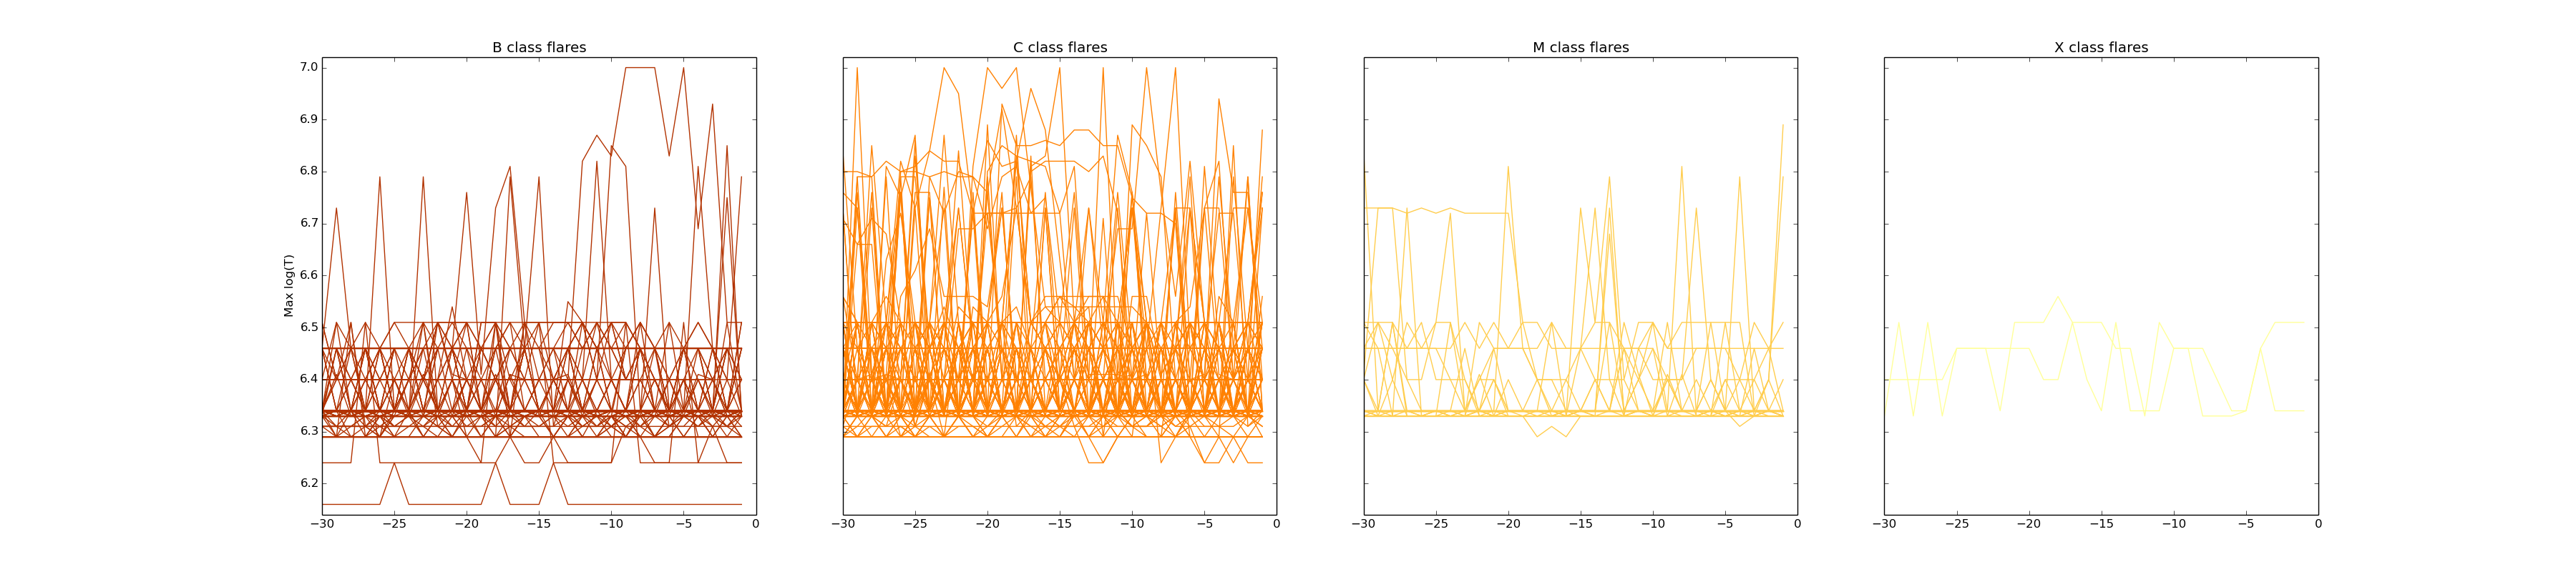
\includegraphics[width=0.7\columnwidth]{tempplotsmax/allars.png}
	\caption{Change in maximum temperature of the corresponding active region plotted for each flare as a function of time before the flare began. Top: maximum temperature against time. Middle: running difference of maximum temperature. Bottom: difference of maximum temperature from maximum temperature at flare start time. Left: B and C class flares, denoted by orange and yellow lines, respectively. Right: M and X class flares, denoted by red and orange lines, repectively.}
	\label{fig:allars_max}
\end{figure}
\begin{figure}
	\centering
		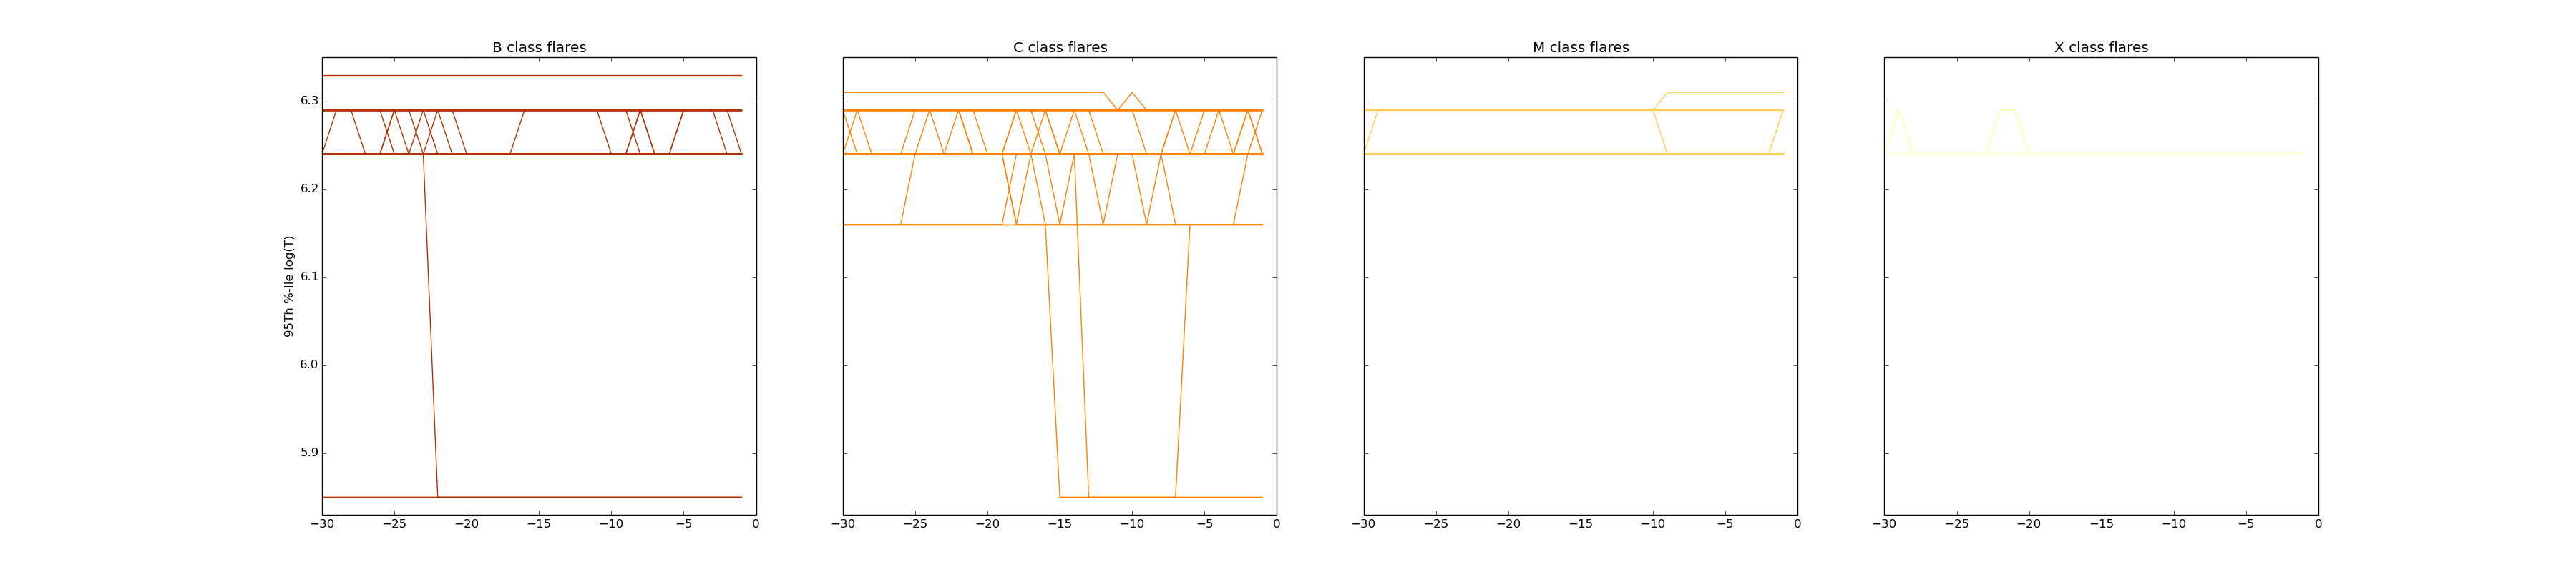
\includegraphics[width=0.7\columnwidth]{tempplots_p95/allars.png}
	\caption{Change in 95th percentile temperature of the corresponding active region plotted for each flare as a function of time before the flare began. Plots and colour-coding are the same as in Figure \ref{fig:allars_max}}
	\label{fig:allars_p95}
\end{figure}
\begin{figure}
	\centering
		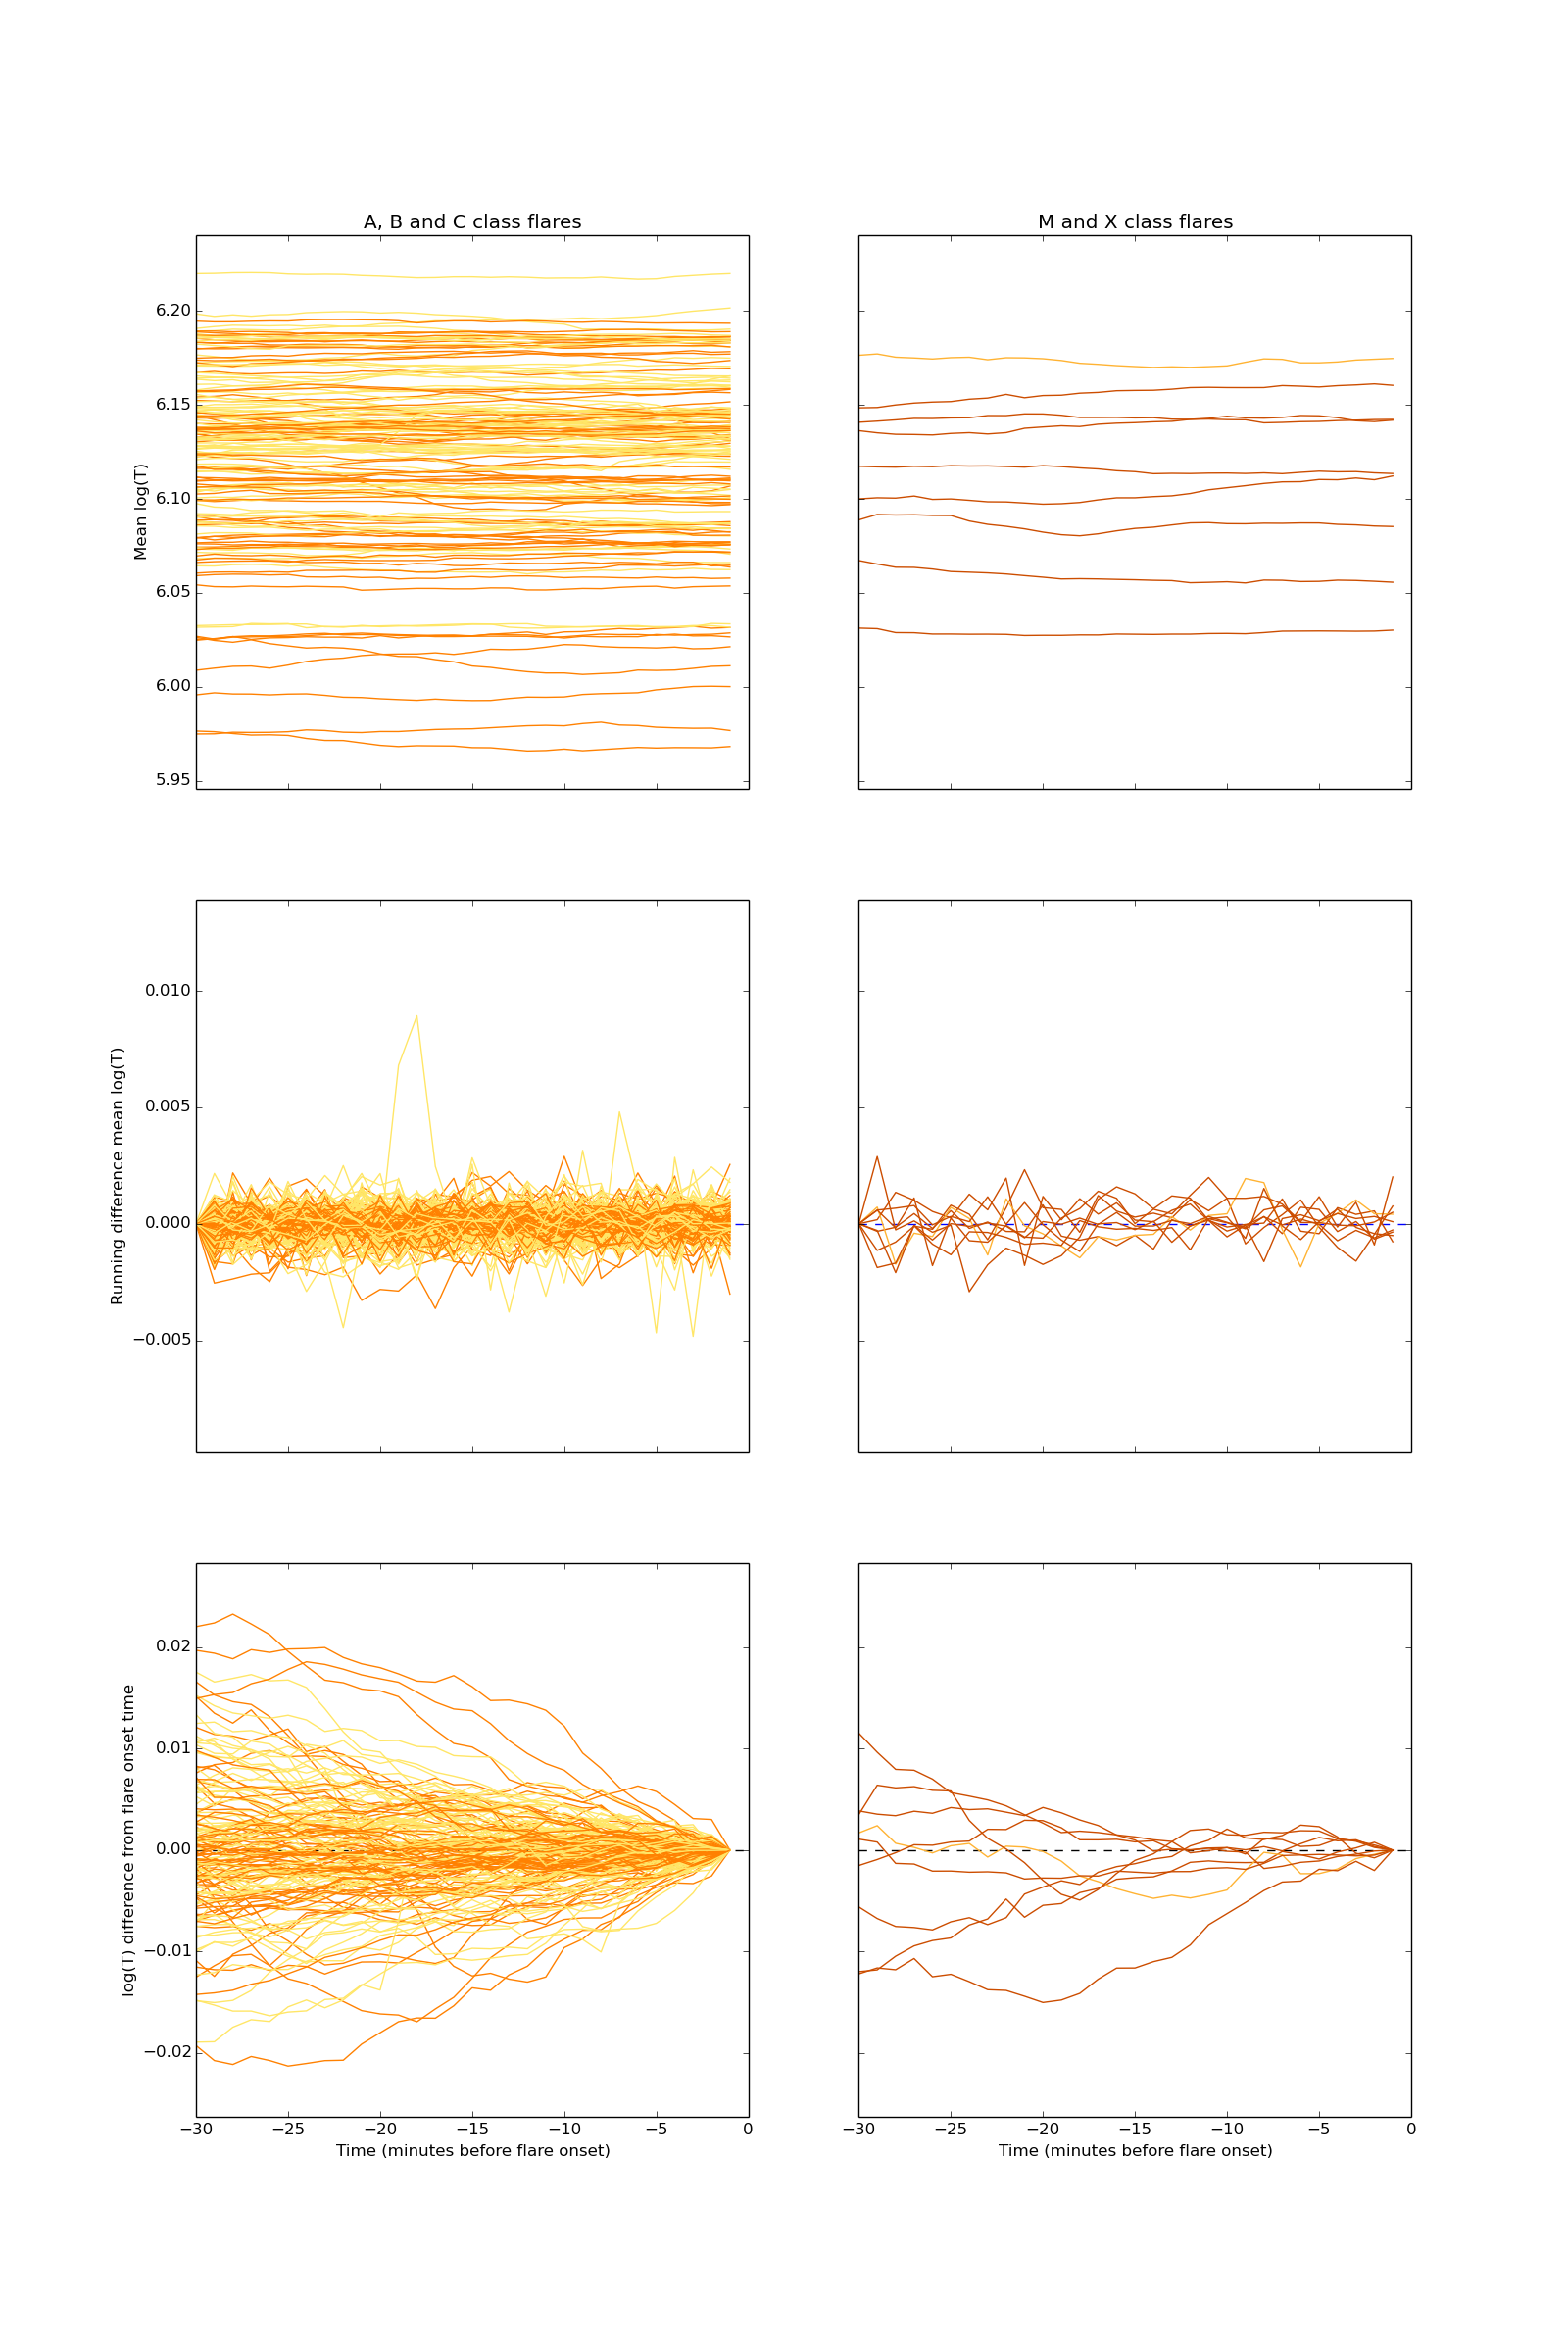
\includegraphics[width=0.7\columnwidth]{tempplotsmean/allars.png}
	\caption{Change in mean temperature of the corresponding active region plotted for each flare as a function of time before the flare began. Plots and colour-coding are the same as in Figure \ref{fig:allars_max}}
	\label{fig:allars_mean}
\end{figure}
\begin{figure}
	\centering
		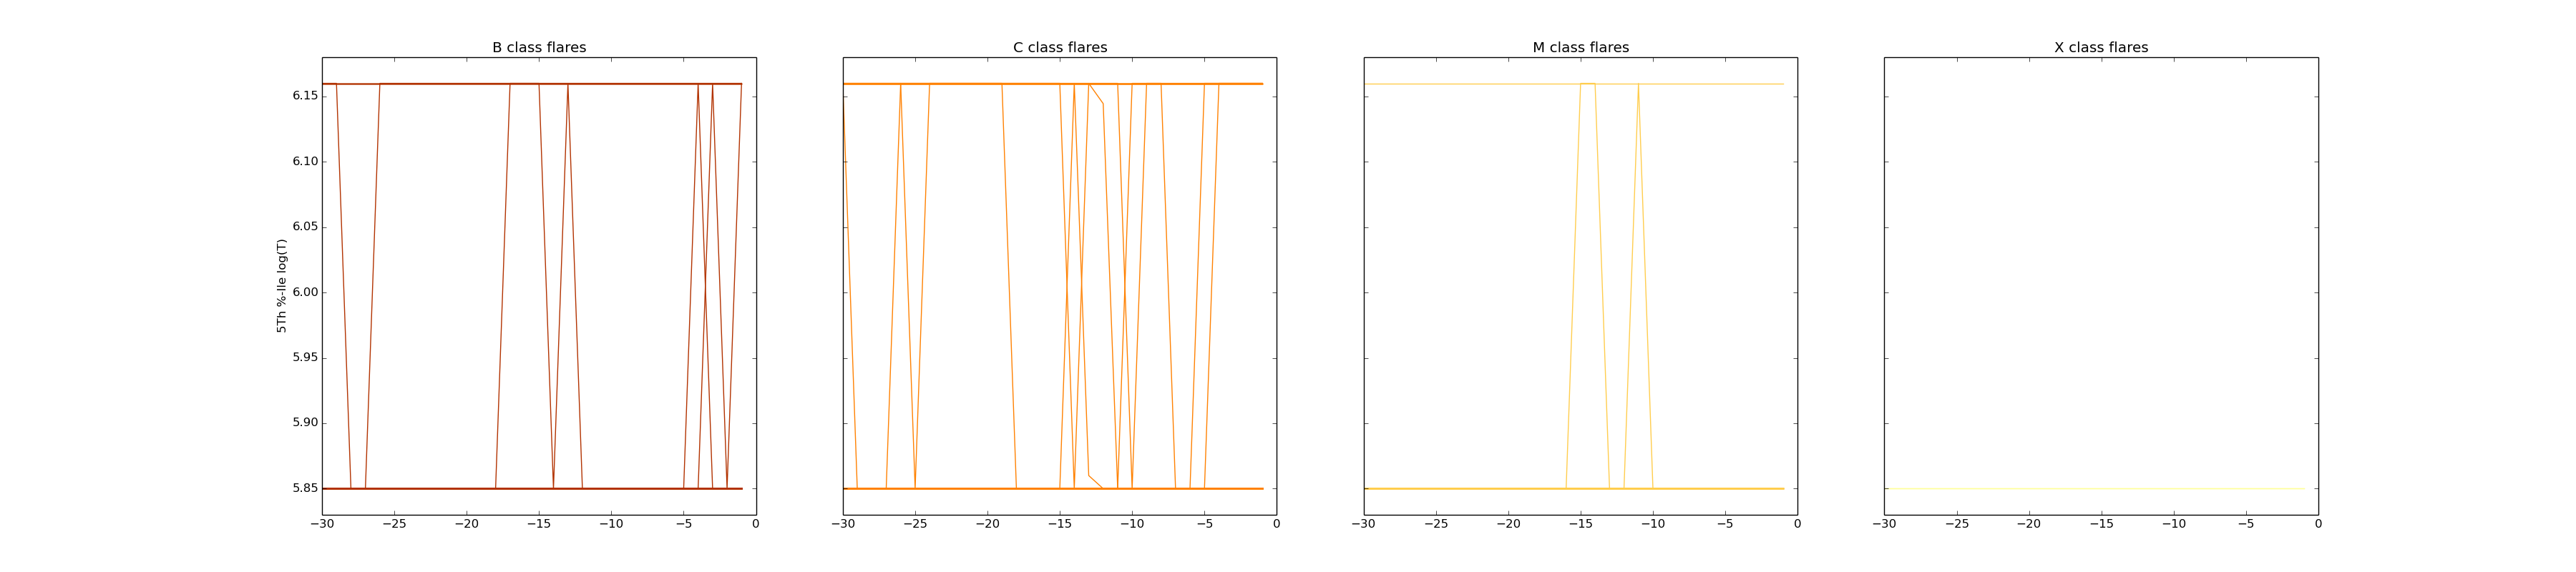
\includegraphics[width=0.7\columnwidth]{tempplots_p5/allars.png}
	\caption{Change in 5th percentile temperature of the corresponding active region plotted for each flare as a function of time before the flare began. Plots and colour-coding are the same as in Figure \ref{fig:allars_max}}
	\label{fig:allars_p5}
\end{figure}
\begin{figure}
	\centering
		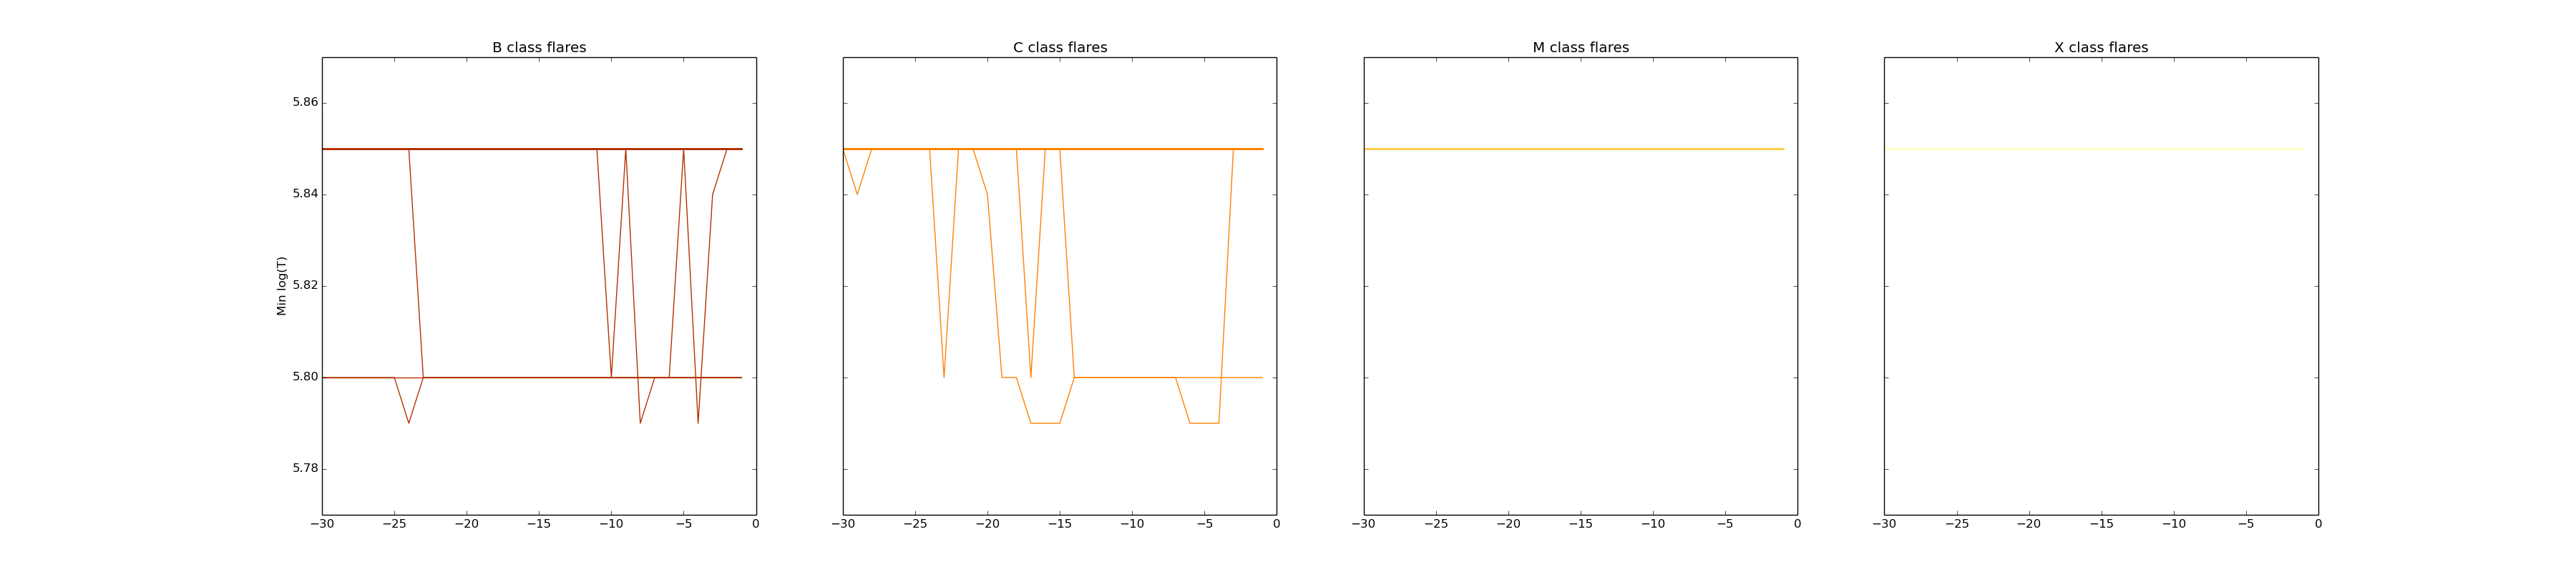
\includegraphics[width=0.7\columnwidth]{tempplots_min/allars.png}
	\caption{Change in minimum temperature of the corresponding active region plotted for each flare as a function of time before the flare began. Plots and colour-coding are the same as in Figure \ref{fig:allars_max}}
	\label{fig:allars_min}
\end{figure}

\subsection{Flare flux vs temperature}
For each temperature parameter, the value for each flare was plotted on a scatter graph against the peak flux of the flare (Figs. \ref{fig:allflares_max}, \ref{fig:allflares_p95}, \ref{fig:allflares_mean}, \ref{fig:allflares_p5} and \ref{fig:allflares_min}).
This was done for four times in each case: 30 minutes before the flare start time, 10 minutes before, 1 minute before and at the flare start time.

% Description of plots for maximum
Figure \ref{fig:allflares_max} shows that the maximum temperatures of the ARs studied are closely grouped around a few temperature values.
This remains the case throughout the 30 minutes before the flare, despite the fact that the temperature of many of these active regions rises and falls significantly during this time.
This sudden increase or decrease of temperature is particularly noticeable in the active regions associated with C class flares, as can also be seen in Figure \ref{fig:allars_max}.

% Description of plots for 95
The scatter graphs in Figure \ref{fig:allflares_p95} show that the 95th percentile temperatures of all the active regions were one of only three or four temperautre values, with no apparent dependence on the peak flux of the associated flare. Most of the active regions remain at a constant temperature for most of the period investigated, with only a few displaying any heating or cooling between the times for which the graphs are plotted.

% Description of plots for mean
The mean temperatures of the active regions are more varied than the other parameters, with values ranging between $log(T) \approx 5.95$ and $log(T) \approx 6.25$. 
Most active regions show no clear link between mean temperature and flare flux, with points being distributed quite uniformly on the plot.
However, it may be worth noting that the flare with the highest flux corresponds to an active region with a temperature near the top of the range shown, while some of the weakest flares correspond to the coolest active regions.
The mean temperature of many of the active regions fluxuates somewhat, but any changes are quite small and the overall distribution of the plots remains largely the same.

% Description of plots for 5
The 5th pecentile temperatures of the active regions were found to be grouped into to distinct temperatures, with no apparent dependence on flux.
A few active regions heat or cool over the time studied, but most remain the same temperature throughout.
The hotter of the temperatures found was only present in active regions corresponding to B and C class flares, as can also be seen in Figure \ref{fig:allars_p5}.

% Description of plots for minimum
Figure \ref{fig:allflares_min} shows that all active regions studied had a minimum temperature of log(T) = 5.85 regardless of the flux of the flare produced.
All active regions appear to remain a constant temperature throughot the time studied.

\begin{figure}
	\centering
		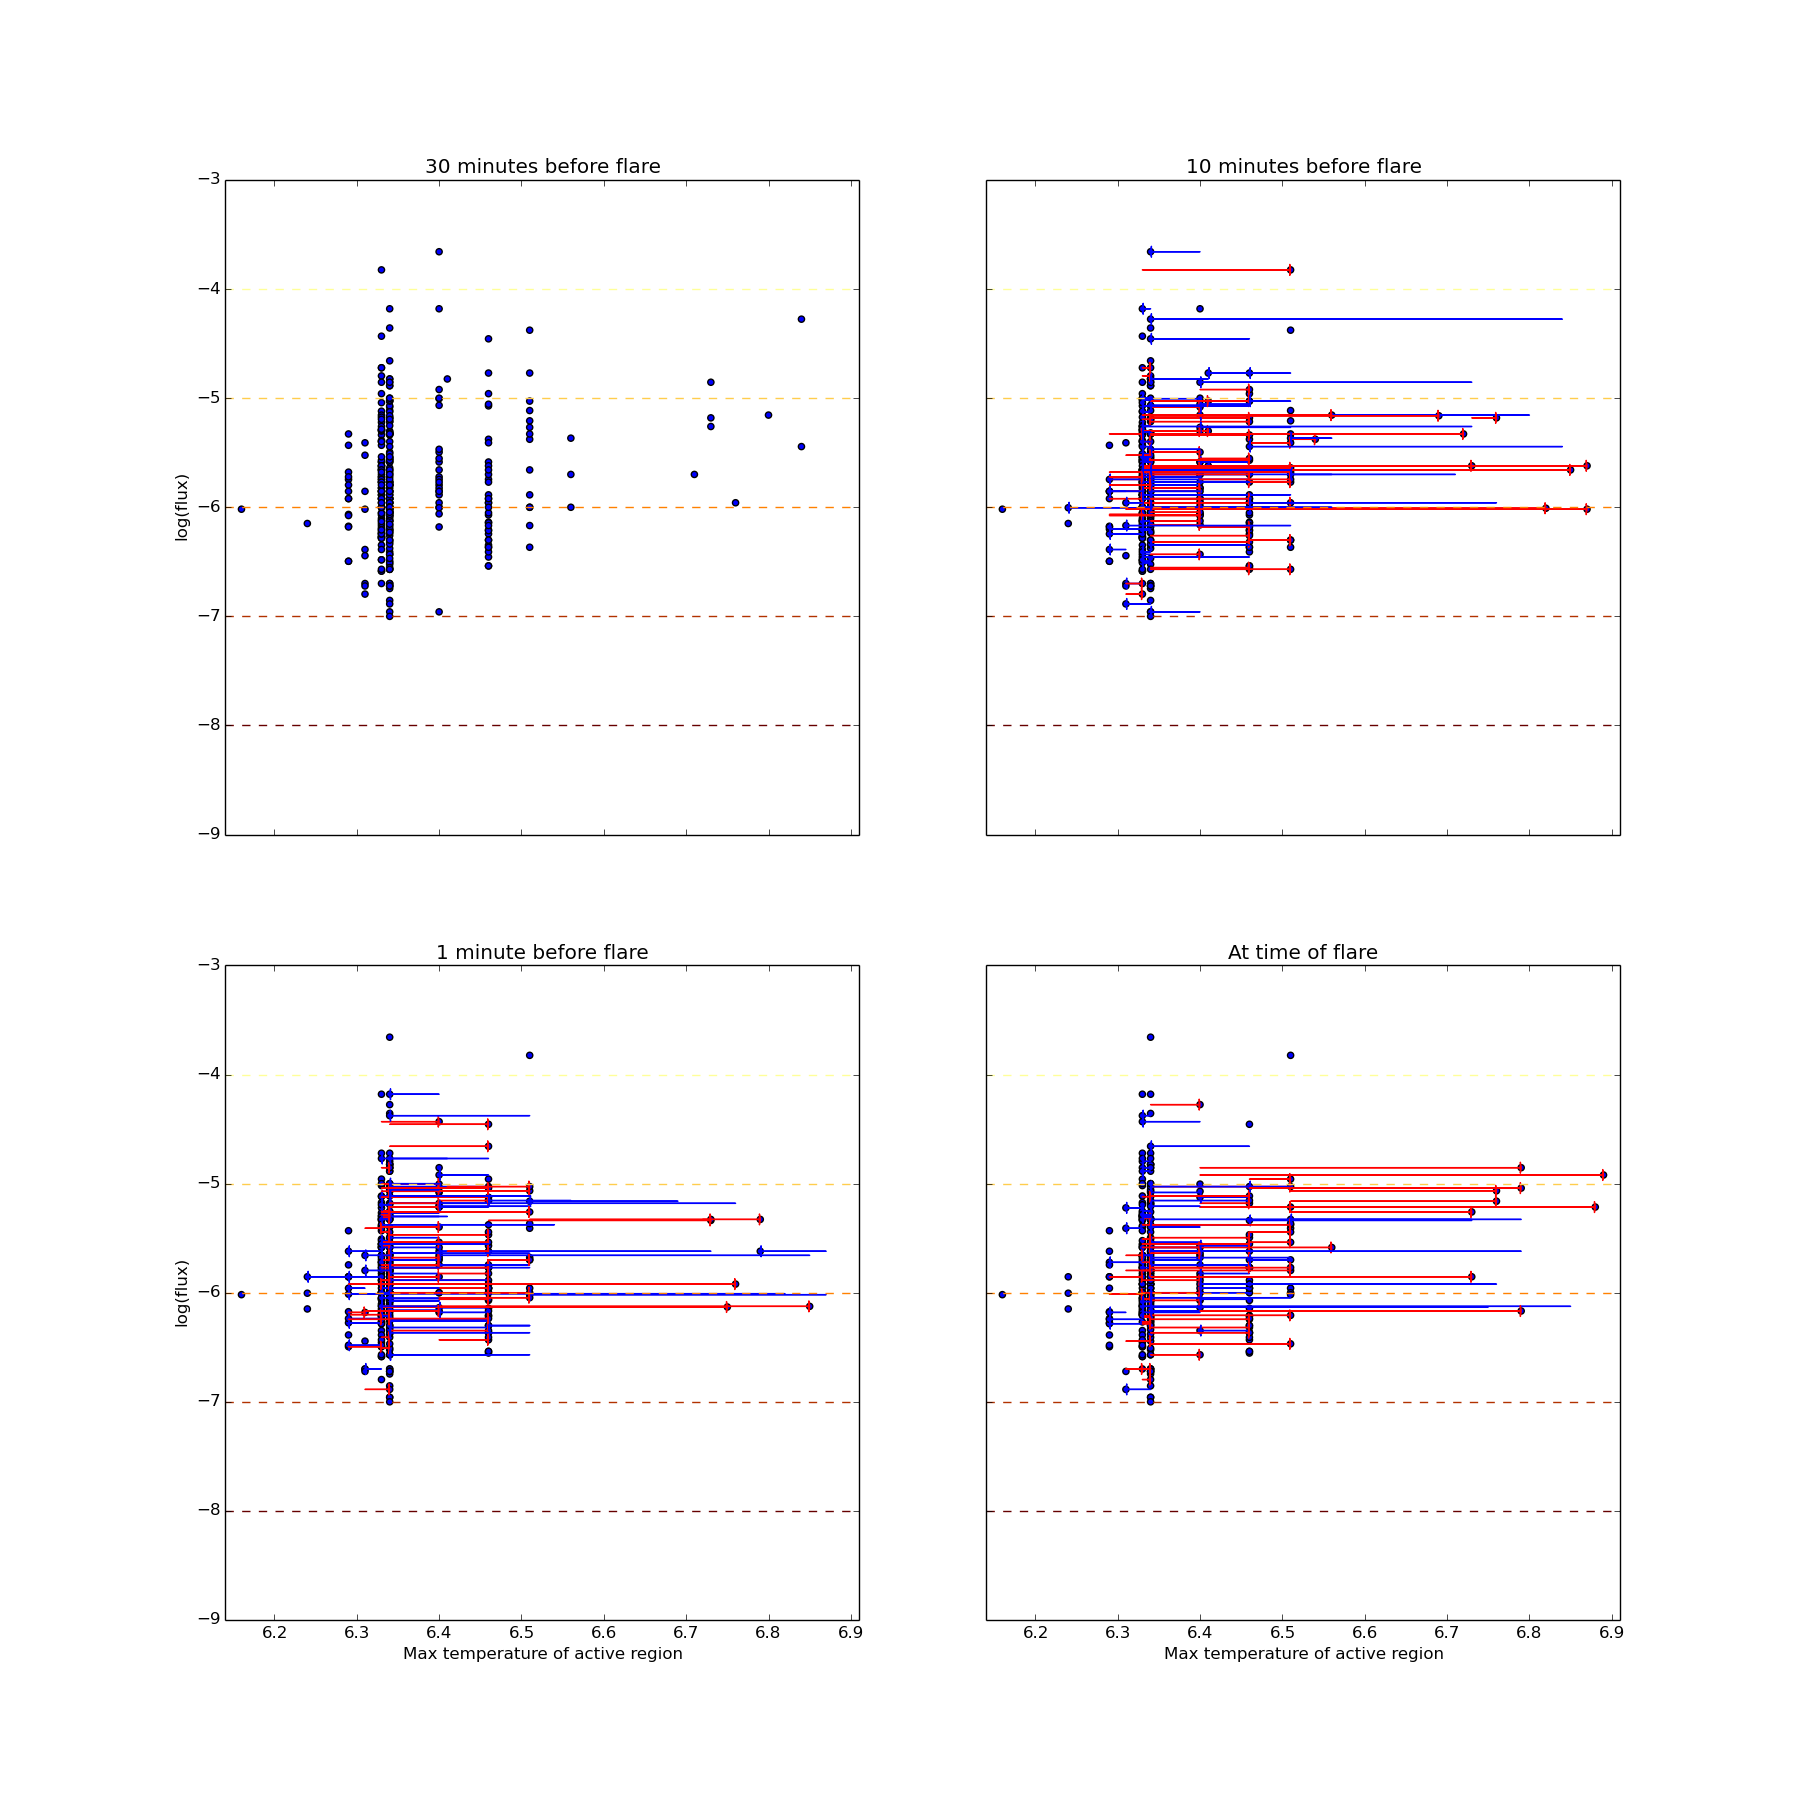
\includegraphics[width=0.9\columnwidth]{tempplotsmax/allflares.png}
	\caption{Scatter graph of flare peak flux against active region maximum temperature for four different times. Top left: 30 minutes before flare start time. Top right: 10 minutes before flare start time. Bottom left: 1 minute before flare start time. Bottom right: flare start time. The red and blue arrows indicate the amount by which the temperature of each active region rose or fell respectively since the time of the previous plot. In each plot the dashed lines indicate the lower thresholds for A, B, C, M and X class flares.}
	\label{fig:allflares_max}
\end{figure}
\begin{figure}
	\centering
		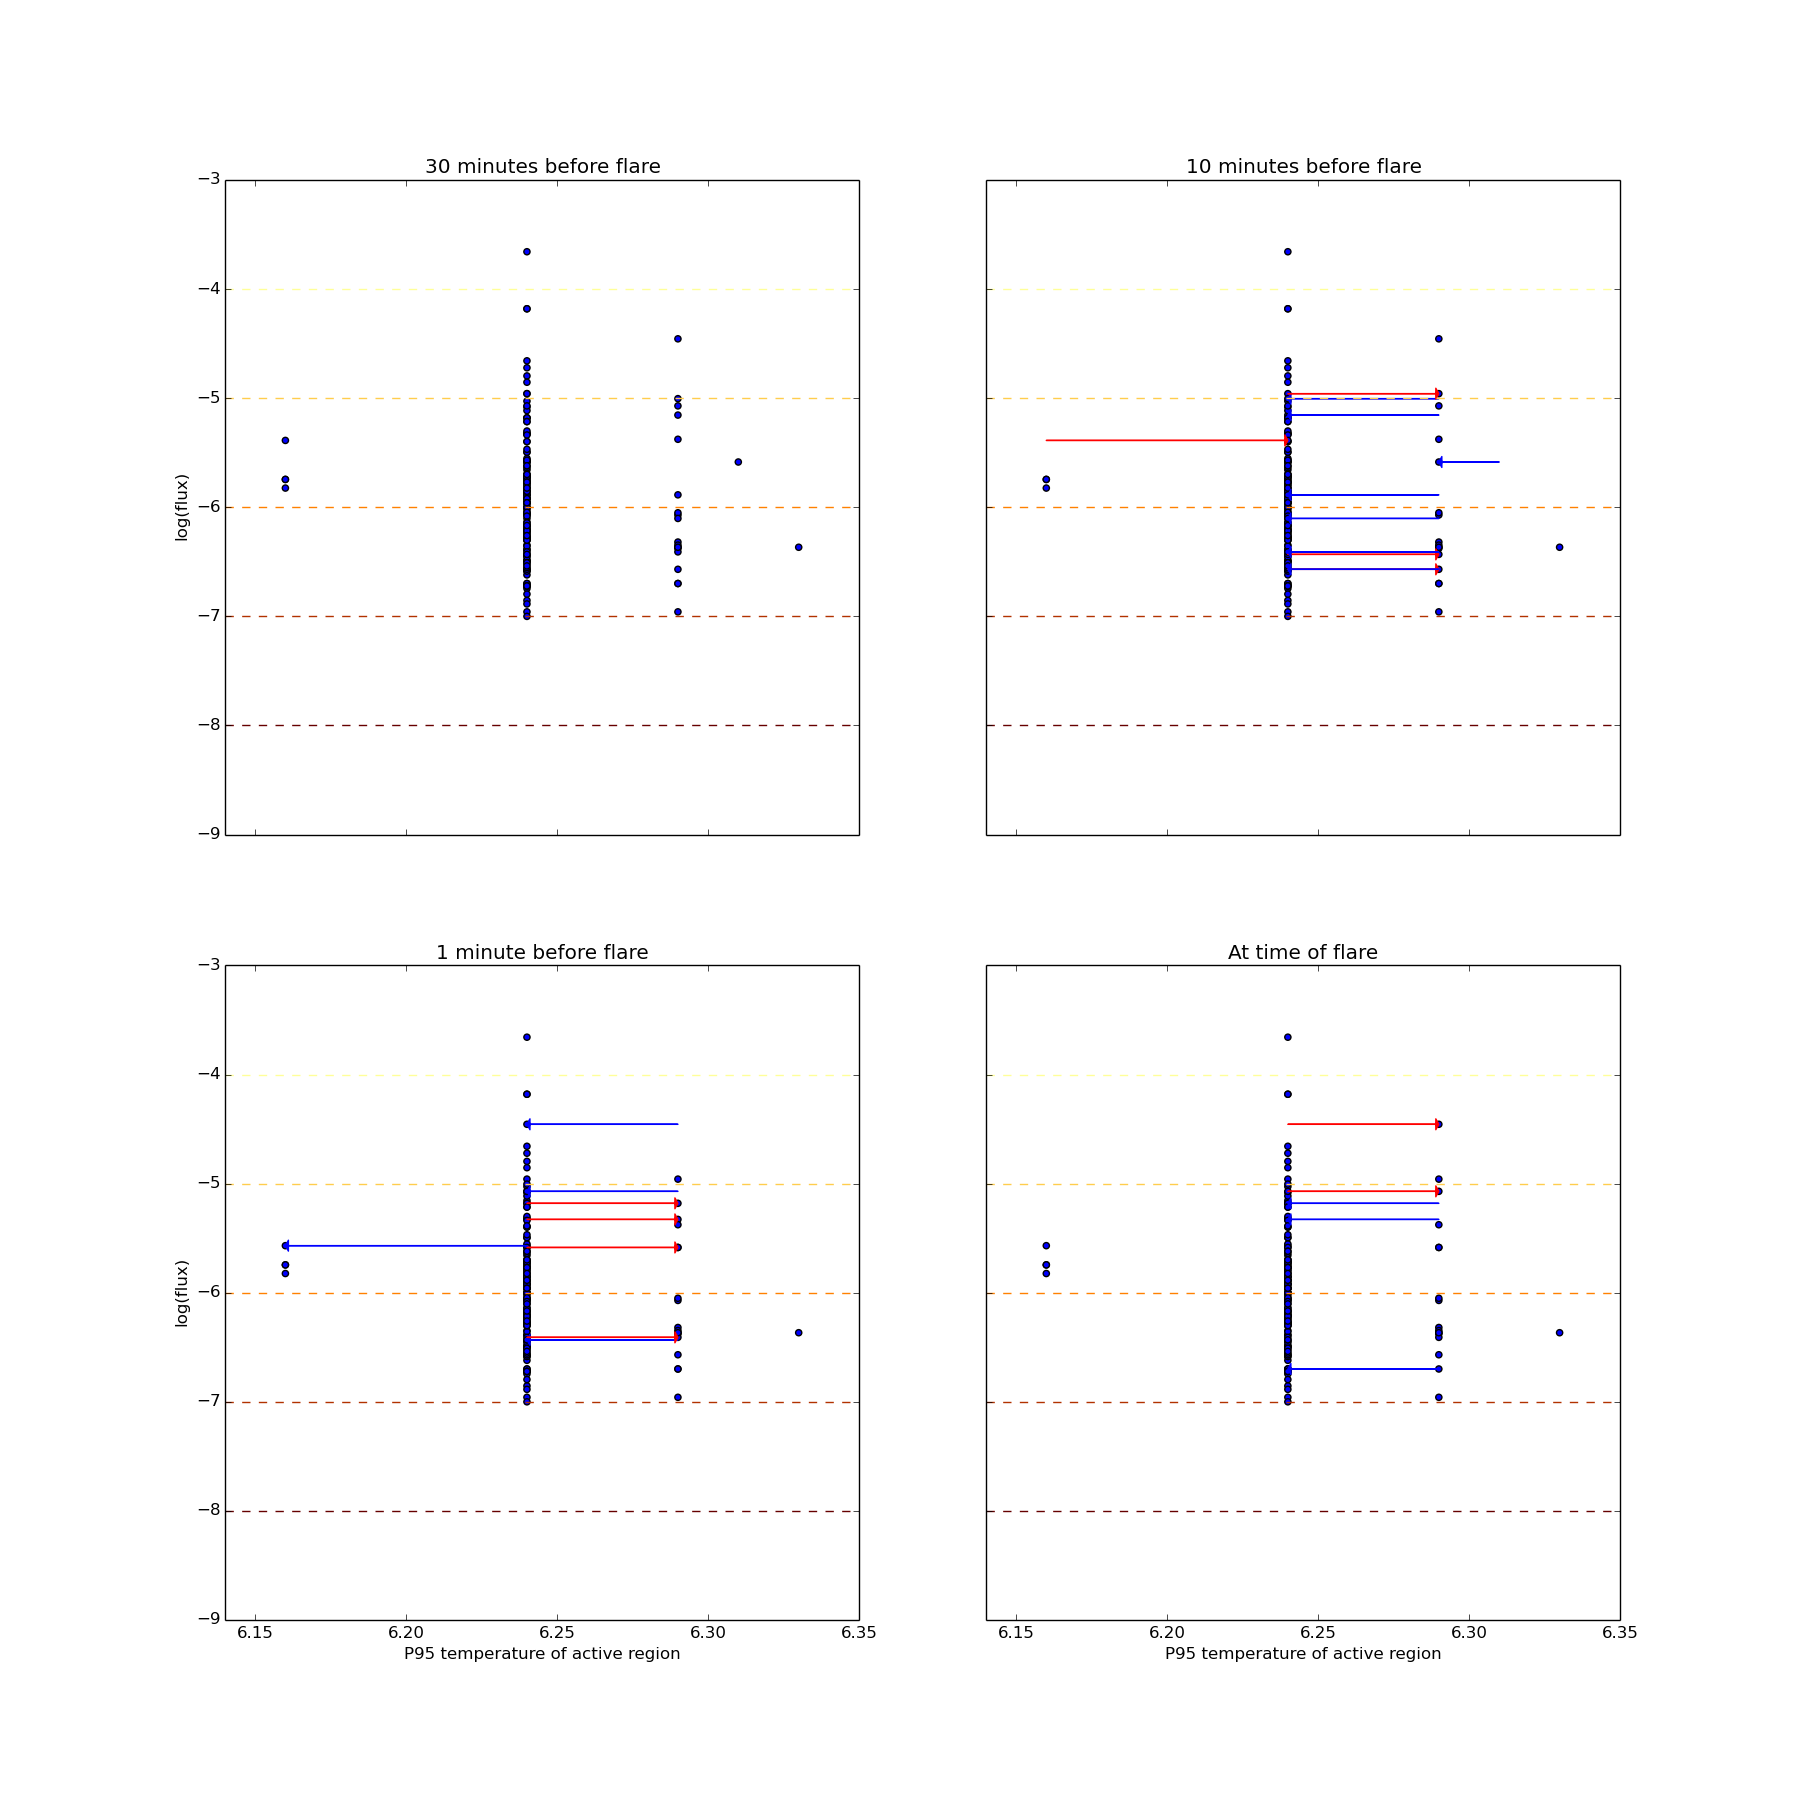
\includegraphics[width=0.9\columnwidth]{tempplots_p95/allflares.png}
	\caption{Scatter graph of flare peak flux against 95th percentile temperature of the corresponding active regions for the same four times as in Figure \ref{fig:allflares_max}.}
	\label{fig:allflares_p95}
\end{figure}
\begin{figure}
	\centering
		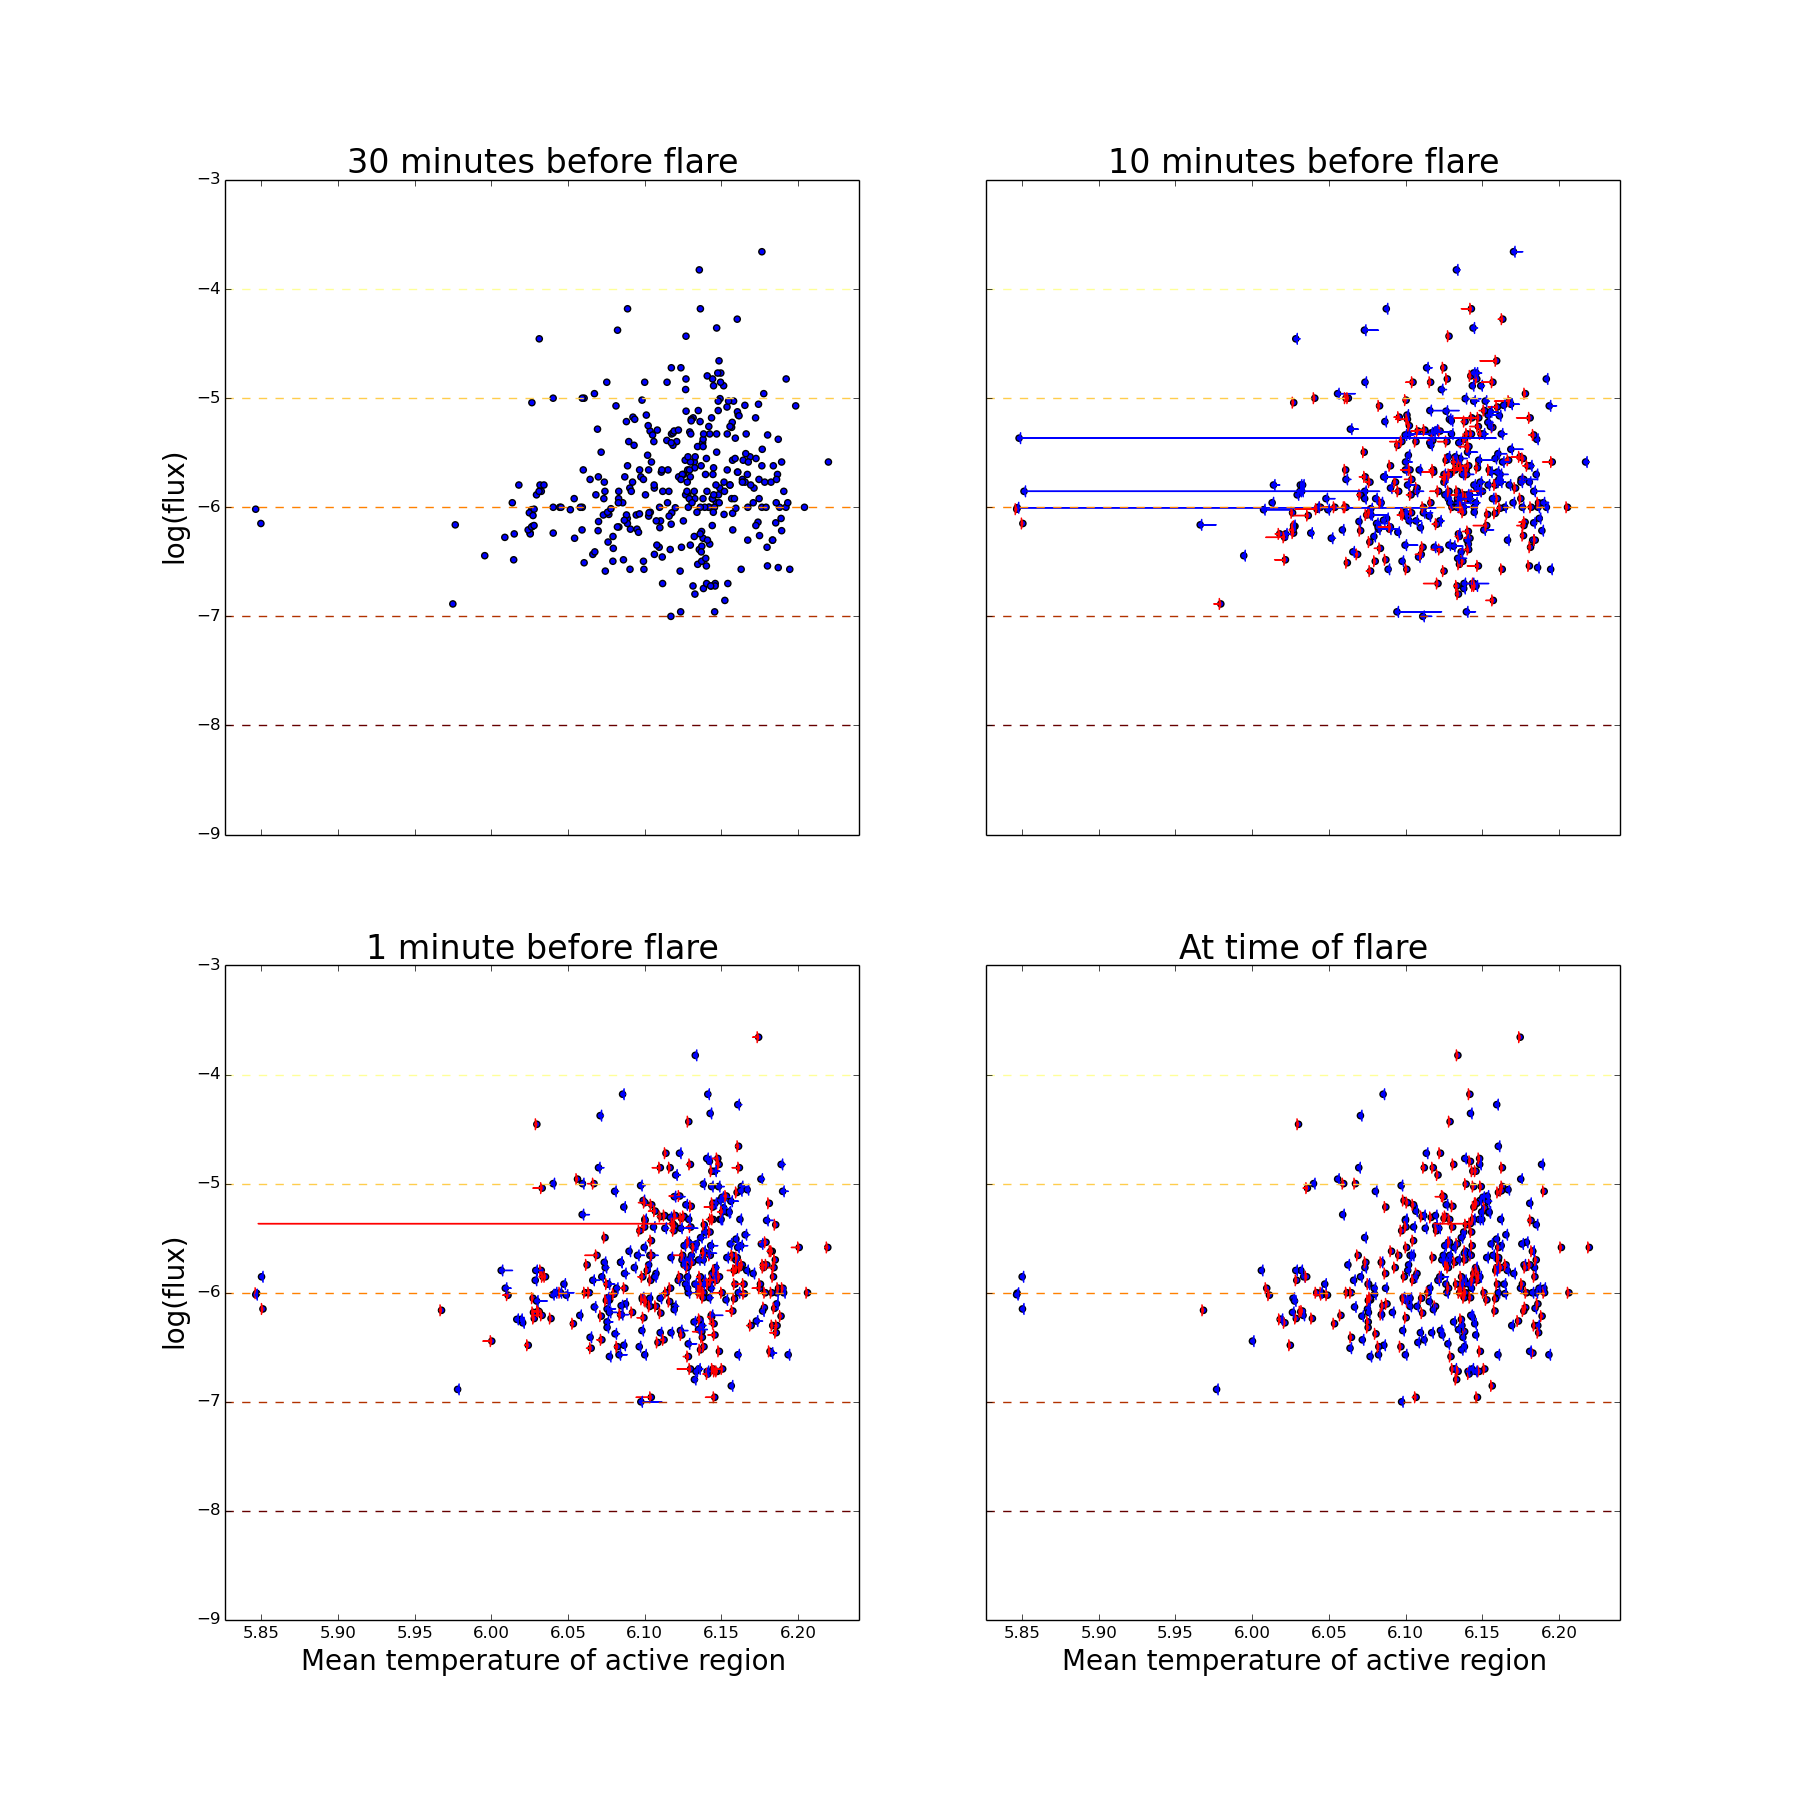
\includegraphics[width=0.9\columnwidth]{tempplotsmean/allflares.png}
	\caption{Scatter graph of flare peak flux against mean temperature of the corresponding active regions for the same four times as in Figure \ref{fig:allflares_max}.}
	\label{fig:allflares_mean}
\end{figure}
\begin{figure}
	\centering
		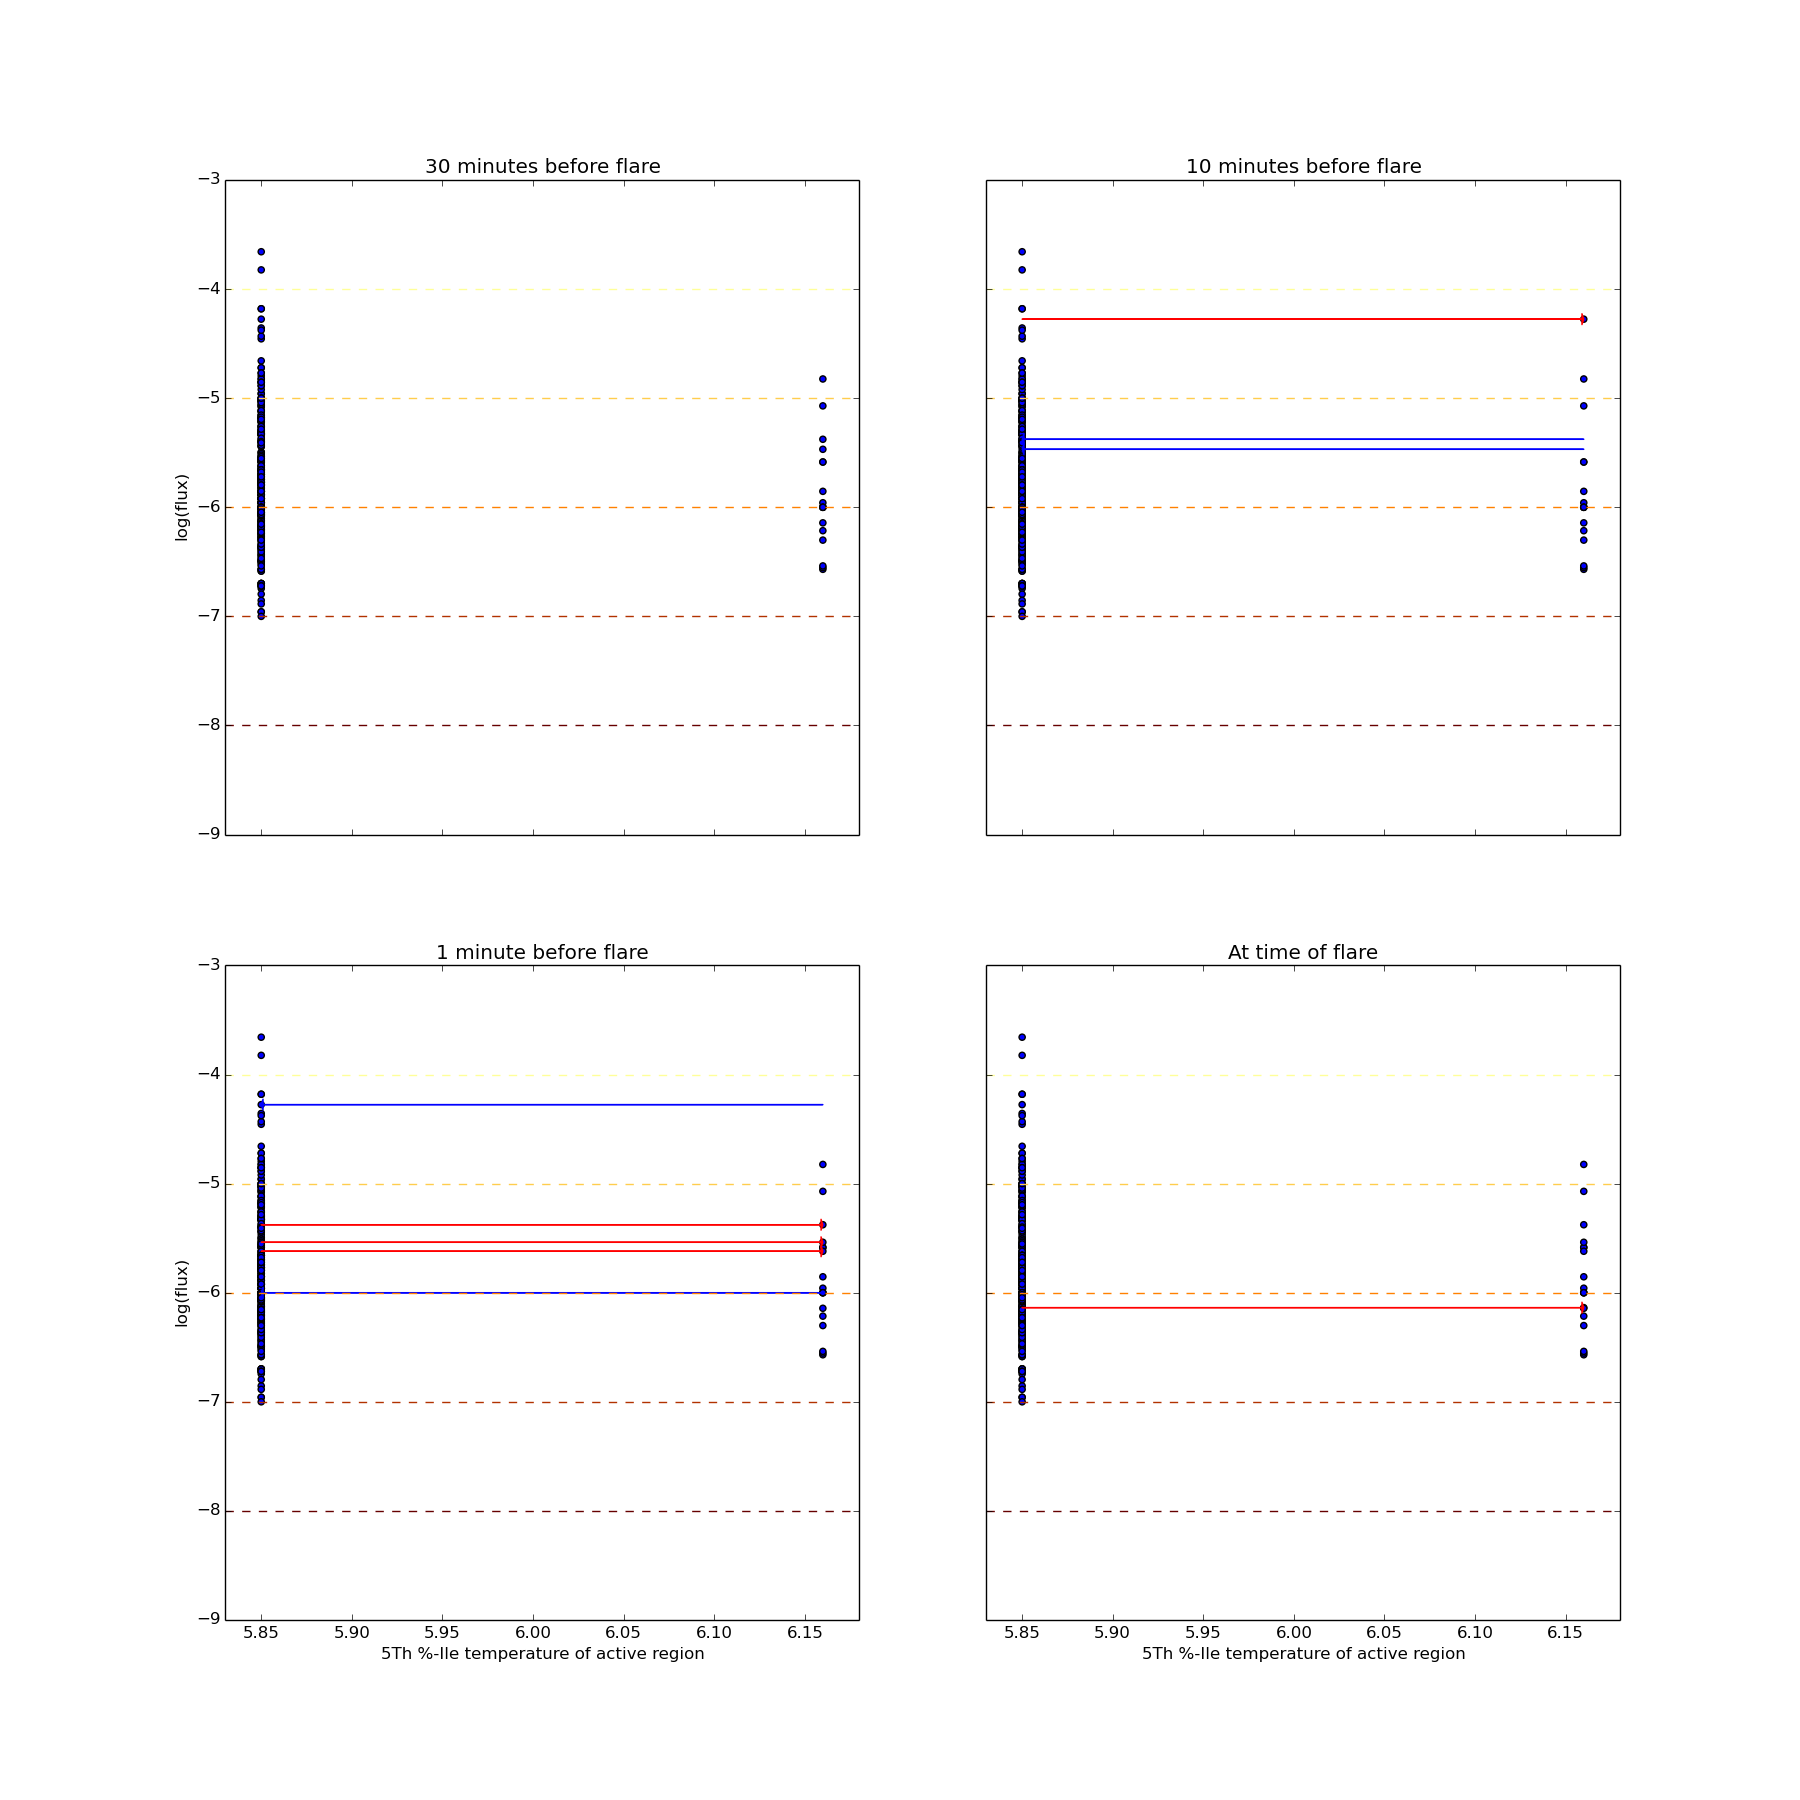
\includegraphics[width=0.9\columnwidth]{tempplots_p5/allflares.png}
	\caption{Scatter graph of flare peak flux against 5th percentile temperature of the corresponding active regions for the same four times as in Figure \ref{fig:allflares_max}.}
	\label{fig:allflares_p5}
\end{figure}
\begin{figure}
	\centering
		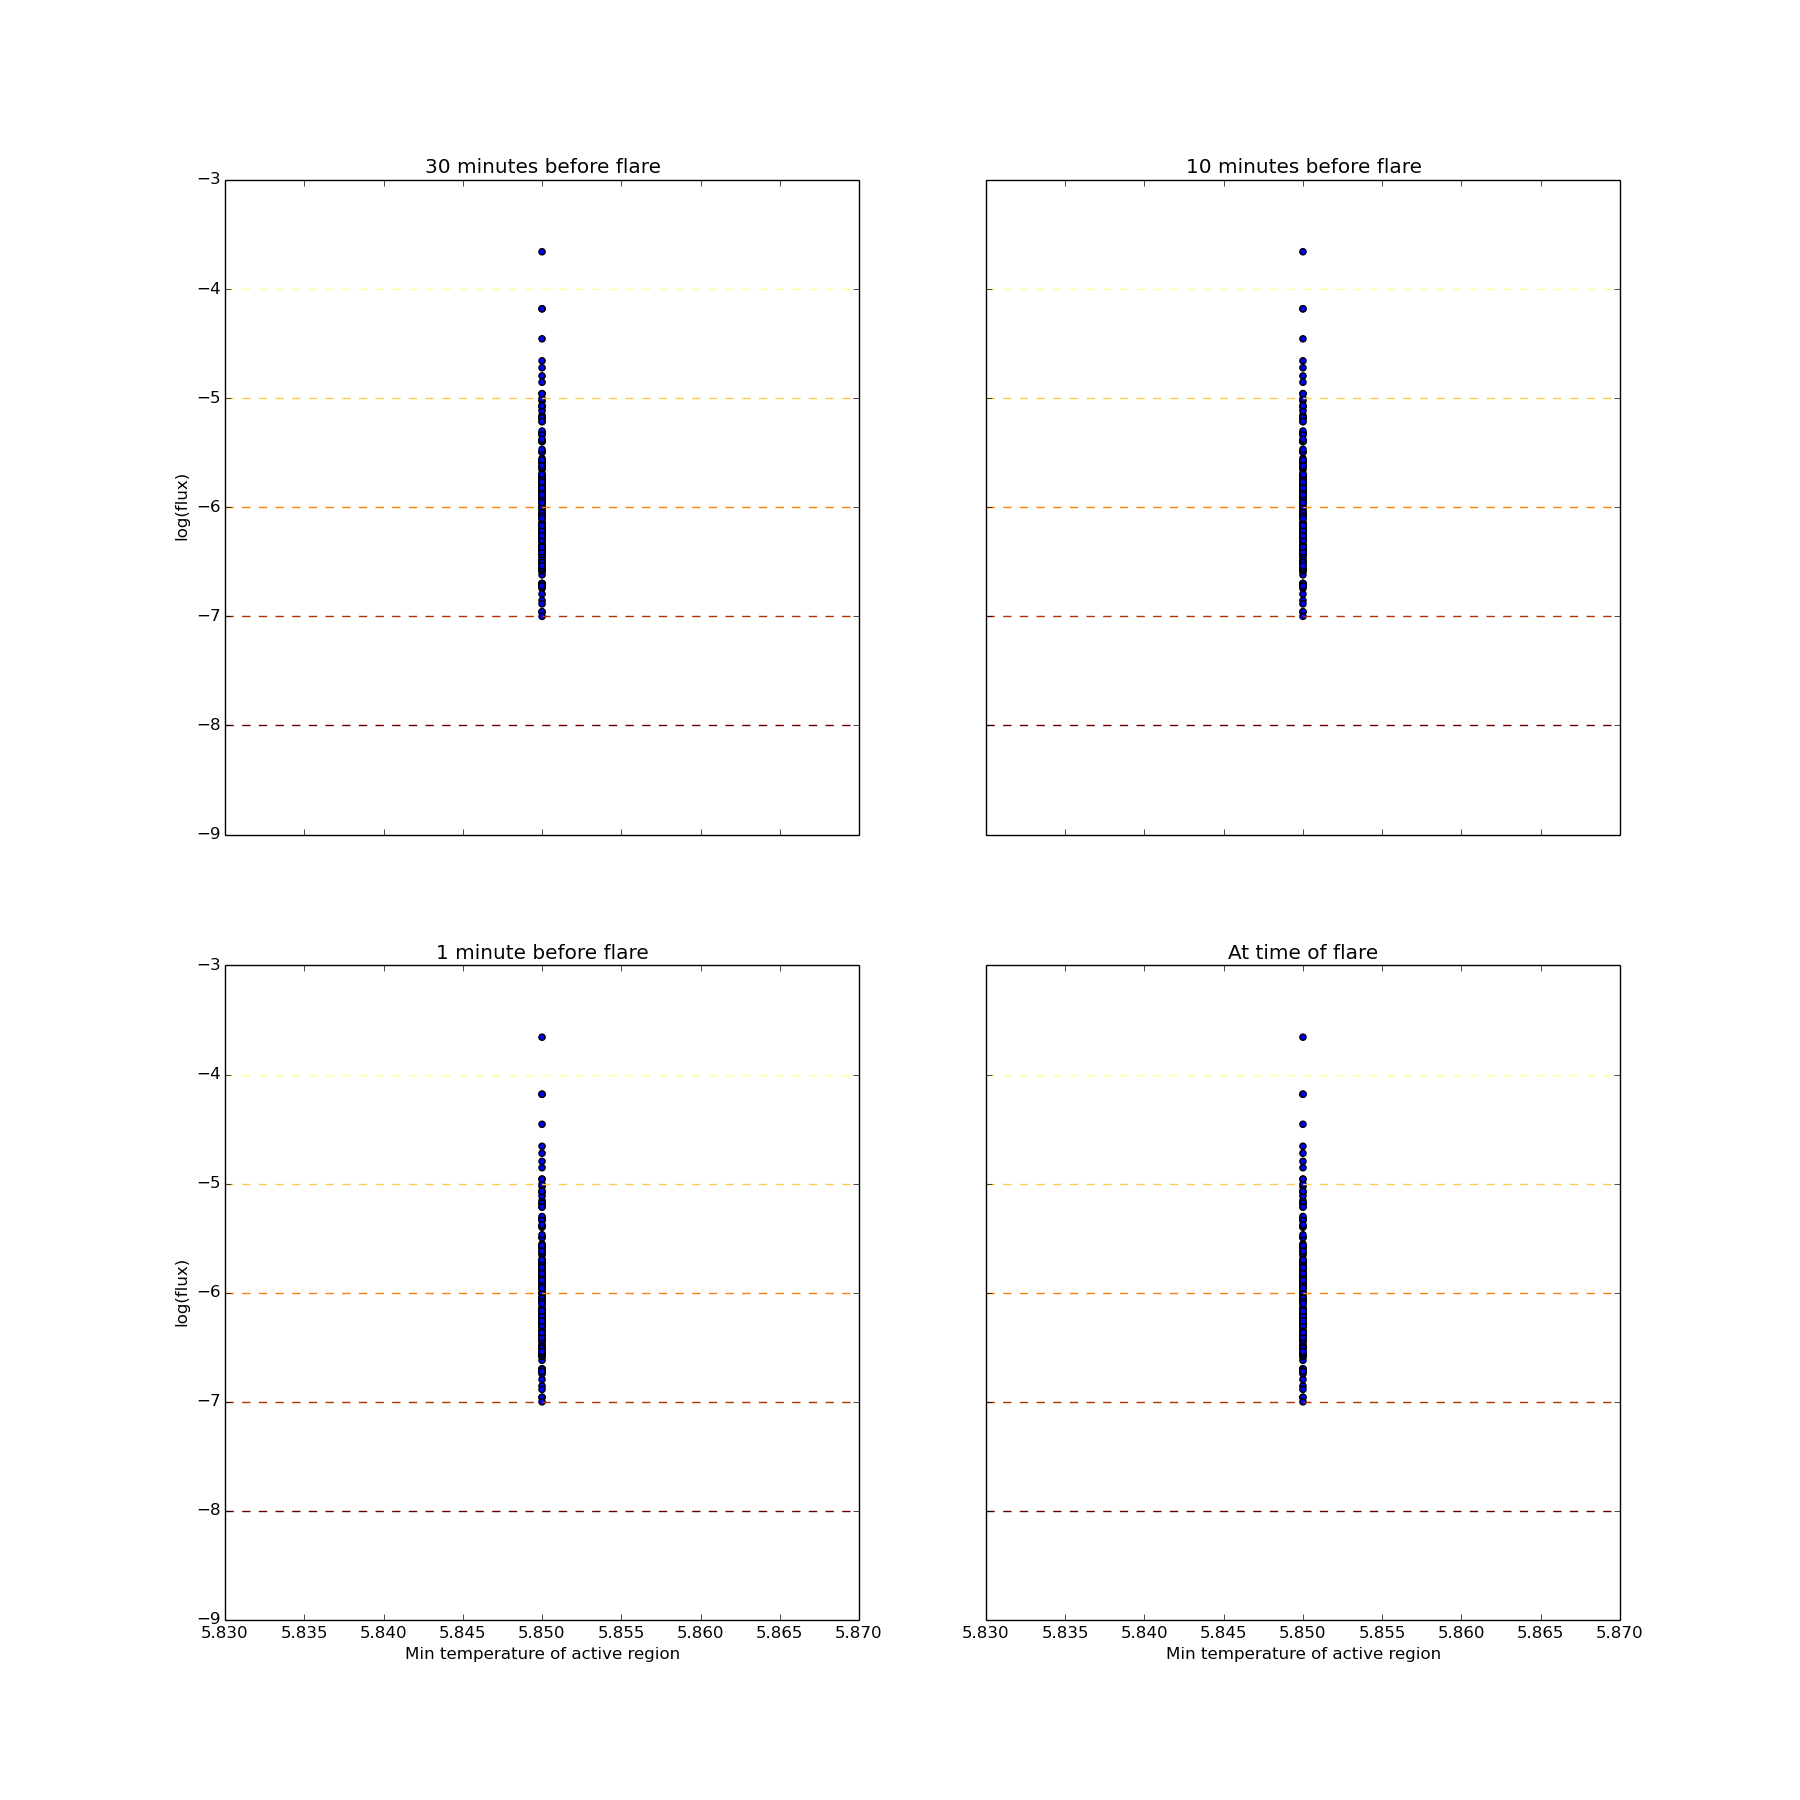
\includegraphics[width=0.9\columnwidth]{tempplots_min/allflares.png}
	\caption{Scatter graph of flare peak flux against minimum temperature of the corresponding active regions for the same four times as in Figure \ref{fig:allflares_max}.}
	\label{fig:allflares_min}
\end{figure}


%===========================================================================
\section{Discussion and conclusions}
From this study, it appears that there is no clear link between solar flares and coronal temperatures.
This is probably mostly due to the relatively small number of flares studied - a much larger sample size would have to be used to properly determine any link or lack thereof.
In particular, this study only included a single X class flare, which as the most energetic are the kind we would most wish to predict.
Future works should therefore aim to consider more large flares.
Non-flaring active regions should also be taken into account and compared against the results presented here.
However, this work does demonstrate that it is now possible to study temperature distributions of the corona in high resolution and on short timescales using fast temperature analysis tools such as the one described in Paper 1.

Figures \ref{fig:allars_max} - \ref{fig:allars_min} show that there is no clear trend in any of the temperature parameters investigated before flares occur.
However, this study only looks at quite a short amount of time before flares; an investigation into longer-term temperature distributions may yield better results.

Similarly, no clear correlation can be seen between peak flare flux and active region temperature, but a much larger sample of flares is needed in order to properly determine whether or not a link exists between the two.
Some of the points on Figure \ref{fig:allflares_mean} do appear to show a rise in temperature with peak flare flux, but the sample size is too small and there are too many other points which do not show such a relation for this to be considered a positive result.

Finally, it is worth remembering that this study only looks at the bulk properties of the active region temperatures.
Any temperature changes leading up to flares may occur on the scale of only a few pixels.
For this reason, the full distribution of temperatures in the active region should be investigated in detail in a future study.

%===========================================================================
\begin{acknowledgements}
	This research has made use of SunPy, an open-source and free community-developed solar data analysis package written in Python \citep{Mumford2013}.
\end{acknowledgements}

%===========================================================================
%\section*{Annexes}

%===========================================================================
\bibliography{C:/Users/Drew/Dropbox/Thesis/thesis_refs,C:/Users/Drew/Documents/library}

\end{linenumbers}
\end{document}